
\documentclass[11pt]{article}
\usepackage[margin=1in]{geometry}
\usepackage{amsmath,amssymb,amsfonts,amsthm,mathtools}
\usepackage{booktabs,longtable,array,multirow}
\usepackage{enumitem}
\usepackage{graphicx}
\usepackage{xcolor}
\usepackage{hyperref}
\usepackage{tikz}
\usetikzlibrary{arrows.meta,positioning,fit,shapes,calc}
\usepackage{microtype}
\usepackage{fancyvrb}
\usepackage{titlesec}
\hypersetup{colorlinks=true,linkcolor=blue!50!black,citecolor=blue!50!black,urlcolor=blue!50!black}
\setlist[itemize]{leftmargin=1.4em,itemsep=0.2em,topsep=0.2em}
\setlist[enumerate]{leftmargin=1.6em,itemsep=0.2em,topsep=0.2em}
\newtheorem{theorem}{Theorem}[section]
\newtheorem{proposition}[theorem]{Proposition}
\newtheorem{lemma}[theorem]{Lemma}
\newtheorem{corollary}[theorem]{Corollary}
\theoremstyle{definition}
\newtheorem{definition}[theorem]{Definition}
\newtheorem{example}[theorem]{Example}
\newtheorem{objective}[theorem]{Objective}
\theoremstyle{remark}
\newtheorem{remark}[theorem]{Remark}
\newcommand{\T}{\mathbb{T}}
\newcommand{\R}{\mathbb{R}}
\newcommand{\Z}{\mathbb{Z}}
\newcommand{\N}{\mathbb{N}}
\newcommand{\C}{\mathbb{C}}
\newcommand{\K}{\mathbb{K}}
\newcommand{\val}{\operatorname{val}}
\newcommand{\Log}{\operatorname{Log}}
\newcommand{\argmax}{\operatorname*{arg\,max}}
\newcommand{\argmin}{\operatorname*{arg\,min}}
\newcommand{\softmax}{\operatorname{softmax}}
\newcommand{\Supp}{\operatorname{Supp}}
\newcommand{\Hom}{\operatorname{Hom}}
\newcommand{\Ext}{\operatorname{Ext}}
\newcommand{\Tor}{\operatorname{Tor}}
\newcommand{\rank}{\operatorname{rank}}
\newcommand{\dist}{\operatorname{dist}}
\newcommand{\bits}{\ensuremath{\operatorname{bits\text{-}per\text{-}byte}}}
\newcommand{\cost}{\operatorname{cost}}
\newcommand{\ctx}{\mathcal{C}}
\newcommand{\Mem}{\mathcal{M}}
\newcommand{\KG}{\mathcal{G}}
\newcommand{\DB}{\mathcal{D}}
\newcommand{\LC}{L_C}
\newcommand{\eps}{\varepsilon}
\newcommand{\one}{\mathbf{1}}
\newcommand{\oplusT}{\oplus}
\newcommand{\otimesT}{\otimes}
\title{\bfseries TropicalGT III:\\ Valuated Context Protocols, Tropical Memory Graphs, and Long-Context Retrieval for Graph-Token Reasoning Agents}
\author{Amelie Schreiber}
\date{June 2026}
\begin{document}
\maketitle

\begin{abstract}
TropicalGT I studied tropical attention as a max-plus inductive bias for graph-token reasoning: dynamic-programming recurrences, shortest-path-like routing, active-face diagnostics, and bits-per-byte-safe auxiliary losses. TropicalGT II extended that view from a single attention layer to iterative reasoning dynamics, tropical algebraic geometry, amoebas, non-Archimedean limits, Viro patchworking, and persistent polyhedral training. This third paper moves the theory to the external substrate of modern agents: model context protocols, markdown memory, knowledge graphs, long-context windows, vector databases, graph-structured retrieval, and projected retrieval heads. The main object is a valuated context graph whose nodes are protocol events, memory blocks, knowledge-graph entities, retrieved chunks, verifier states, and generated reasoning packets. Each node carries a dense embedding, a tropical valuation vector, a provenance/security type, adjacency data, and optional topological or algebraic certificates. Retrieval is no longer a flat nearest-neighbor query; it is a tropical graph operation that combines max-plus attention, graph adjacency expansion, sheaf gluing, valuation-compatible quantization, and finite audit codes. We develop definitions, theorem/proof statements, practical training objectives, pseudocode, and implementation guidance for building an efficient graph-structured vector database and a learned projected retrieval head. The training criterion remains deployment-oriented: every memory code, graph edge, tropical cache, or auxiliary certificate must pay for itself by improving held-out \bits, reasoning quality, retrieval accuracy, safety/compliance, or behavior control under explicit artifact-byte accounting.
\end{abstract}

\tableofcontents
\newpage

\section{Introduction}

A reasoning agent is increasingly an algorithm over an external context substrate. It reads a prompt, consults tools, opens resources, invokes model context protocol (MCP) servers, searches a memory store, follows knowledge-graph edges, synthesizes intermediate scratch states, and finally emits an answer. In a small language model this substrate is often implicit. In a long-context agent it becomes an explicit data structure: a 1--10M token canvas populated by protocol observations, markdown memories, retrieved documents, entity neighborhoods, verifier traces, and generated reasoning blocks. A theory of reasoning quality must therefore say not only how a transformer updates hidden vectors, but also how the system constructs, compresses, retrieves, and audits the context that the transformer sees.

TropicalGT III develops such a theory. The immediate predecessor, TropicalGT II, treated reasoning trajectories as evolving tropical and polyhedral objects. It used the tropical semifield \(\T=\R\cup\{-\infty\}\) with tropical addition \(a\oplusT b=\max(a,b)\) and tropical multiplication \(a\otimesT b=a+b\), and used tropical hypersurfaces as corner loci of piecewise-linear functions. The tropical algebraic geometry source text frames tropical varieties through logarithmic images, non-Archimedean amoebas, the tropical semifield, tropical curves with integer affine structure, patchworking, and enumerative correspondences \cite{ItenbergMikhalkinShustin}. It also makes explicit the bridge between classical degenerations and tropical limits: amoebas of families converge on compact sets, non-Archimedean amoebas arise by coordinatewise valuations, and the corner locus of a tropical polynomial recovers the tropicalized hypersurface. These are exactly the structures one wants for a long-context memory system: a large continuous computation should have a finite piecewise-linear shadow, and retrieval decisions should be stable under controlled deformations.

The new setting differs from TropicalGT I--II in three ways.

First, the basic token is no longer merely a graph token inside a model layer. It is a typed record in an agent context store. Examples include an MCP tool call, a tool result, a markdown heading, a code block, a knowledge-graph triple, a citation span, a verifier judgment, a refusal rationale, a conversation summary, or a generated reasoning step. The official MCP specification describes MCP as a protocol that connects LLM applications to external data and tools via hosts, clients, and servers, with server features such as resources, prompts, and tools and client features such as roots and sampling \cite{MCP2025}. TropicalGT III treats each such interaction as a node or hyperedge in a context graph.

Second, retrieval is a graph-structured computation. A flat vector database returns nearest chunks. A reasoning memory should return compatible subgraphs: evidence nodes with provenance, tool nodes with permissions, markdown blocks with parent headings, knowledge-graph neighborhoods with relation types, and prior reasoning packets with verifier labels. Thus a retrieved object is not just \(z\in\R^d\), but a tuple
\[
    r_v=(z_v, a_v, q_v, p_v, \tau_v, N(v)),
\]
where \(z_v\) is a dense embedding, \(a_v\) is a tropical or valuated code, \(q_v\) is a quantized code, \(p_v\) is provenance/permission metadata, \(\tau_v\) is type, and \(N(v)\) is an adjacency neighborhood. The vector database therefore stores graph-structured vectors.

Third, the deployed system must be compression-accountable. The central metric is held-out \bits:
\[
\bits(x;\theta)=\frac{-\log_2 p_\theta(x)}{|x|_{\rm bytes}}.
\]
A retrieval cache, projected index, quantizer, tropical support certificate, or graph expansion rule is useful only if it improves held-out \bits, answer accuracy, retrieval quality, safety/compliance, or behavior control after charging artifact bytes and runtime tokens. This discipline was present in the ToricGT papers and in TropicalGT I--II; here it becomes a memory-store design principle.

\paragraph{Contributions.}
This paper gives: (i) a formal definition of valuated context graphs for MCP traces, markdown memory, knowledge graphs, and reasoning packets; (ii) a graph-structured vector database with tropical, dense, sparse, and certificate channels; (iii) a learned projection theory for efficient retrieval heads; (iv) quantization results showing when top-k retrieval and graph expansion are stable under tropical and product-quantized codes; (v) a tropical patchworking view of memory assembly; (vi) sheaf and Cech-style consistency losses for retrieved context; (vii) a long-context execution model in which repeated iterations fill a context window up to \(\LC\le 10^7\) tokens; (viii) a catalogue of training losses, metrics, objectives, and regularizers; and (ix) reproducibility details including data schemas, pseudocode, ablations, and deployment gates.

\paragraph{What this paper is not.}
This is not a claim that an LLM literally stores a tropical variety, nor that MCP systems are algebraic varieties. The claim is operational: tropical and algebraic structures give finite, auditable objects that regularize retrieval, memory compression, context assembly, and reasoning trajectories. They are valuable precisely when they produce measurable utility under a held-out scoring rule.

\section{Background and continuity with TropicalGT I--II}

\subsection{Tropical attention and graph-token reasoning}

TropicalGT I began with the observation that many reasoning computations use \(\max\), \(\min\), and ordinary addition rather than probability averaging. Dynamic programming, shortest paths, transitive closure, alignment, parsing, Viterbi decoding, scheduling, and certain graph search procedures naturally live in idempotent semirings. The NeurIPS 2025 Tropical Attention paper introduces multi-head tropical attention as a max-plus attention mechanism and proves approximation results for tropical circuits and tropical transitive closure \cite{Hashemi2025TA}. The official implementation frames the mechanism as a neural algorithmic reasoning component for combinatorial tasks \cite{TropicalAttentionCode}. TropicalGT I adapted this idea to graph-token agents, adding equivariant tokenization, active-face diagnostics, and bits-per-byte-gated training.

A max-plus tropical attention head computes, for query \(i\) and coordinate \(c\),
\[
    Y_{ic}=\max_{j\in [L]}\{S_{ij}+V_{jc}\}.
\]
The active set \(A_{ic}=\argmax_j(S_{ij}+V_{jc})\) is a certificate: it says which key/value token actually controls the output. The top-two margin
\[
    \Delta_{ic}=z^{(1)}_{ic}-z^{(2)}_{ic},\qquad z_{icj}=S_{ij}+V_{jc},
\]
measures stability. If a perturbation has size smaller than \(\Delta_{ic}/2\), the active predecessor cannot change. This kind of certificate is useful for long-context retrieval because context stores introduce many perturbations: projection, approximate search, quantization, pruning, summary replacement, graph expansion, and security filtering.

\subsection{From layers to tropical geometry}

TropicalGT II extended the attention-level view to a geometric view. A tropical polynomial
\[
    f(x)=\max_{a\in A}\{c_a+\langle a,x\rangle\}
\]
has a corner locus where at least two affine forms tie. The attached tropical geometry book defines tropical hypersurfaces as the non-smooth locus of a tropical polynomial and relates them to tropicalizations over non-Archimedean fields \cite{ItenbergMikhalkinShustin}. The Newton polytope \(\operatorname{Conv}(A)\) and the normal fan govern which affine piece is active. Thus the active pattern of a tropical head is not just an implementation artifact; it is a polyhedral chart.

TropicalGT II then treated iterative reasoning as a dynamical system
\[
    R_0\xrightarrow{F_\theta}R_1\xrightarrow{F_\theta}\cdots\xrightarrow{F_\theta}R_T,
\]
where each state carried a graph-of-thought packet, a filtered simplicial complex, a persistence summary, and tropical chart data. The central lesson was that reasoning trajectories should have stable polyhedral, topological, and algebraic summaries.

\subsection{The third setting: external context as a tropical object}

The next natural step is to move from hidden trajectories to external context. Modern agents have a context substrate with several layers:
\begin{enumerate}
    \item an MCP layer of hosts, clients, servers, resources, prompts, tools, roots, tasks, and protocol messages;
    \item a markdown memory layer of headings, paragraphs, lists, code blocks, links, citations, and summaries;
    \item a knowledge-graph layer of entities, relations, event nodes, provenance, and typed edges;
    \item a vector retrieval layer of dense embeddings, sparse features, product-quantized codes, and graph adjacency;
    \item a long-context layer in which retrieved and generated blocks fill a context window of length \(\LC\).
\end{enumerate}
TropicalGT III unifies these as a valuated context graph.

\begin{figure}[t]
\centering
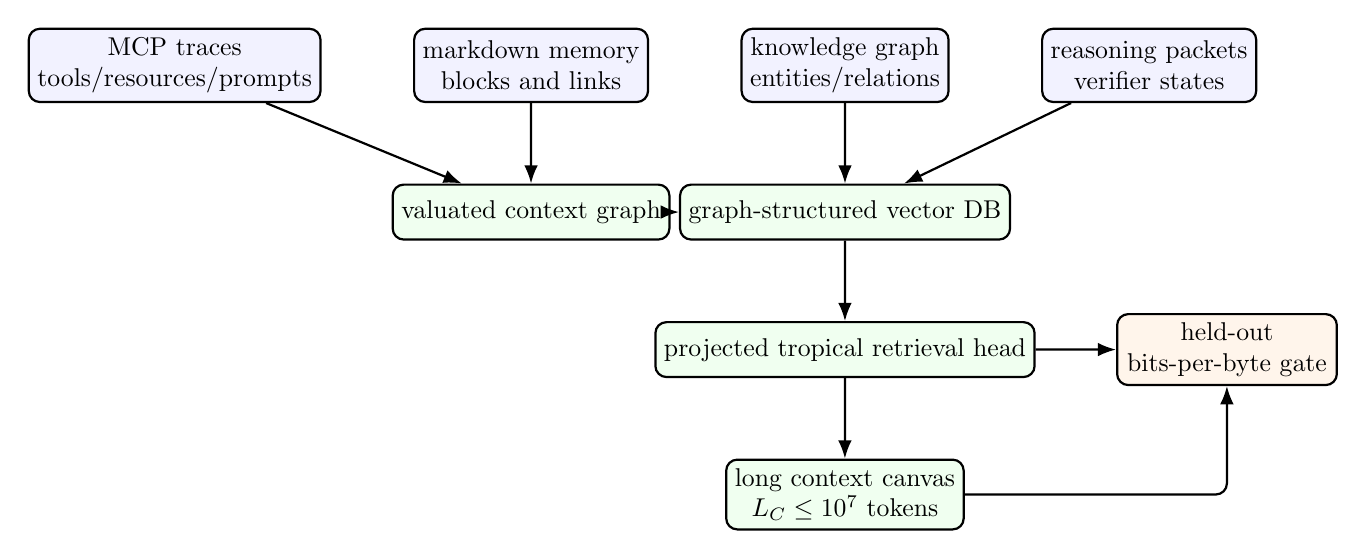
\begin{tikzpicture}[node distance=1.25cm,>=Latex,rounded corners,thick,scale=0.93, every node/.style={transform shape}]
\tikzstyle{box}=[draw, rounded corners, align=center, minimum width=2.7cm, minimum height=1cm, fill=blue!5]
\tikzstyle{smallbox}=[draw, rounded corners, align=center, minimum width=2.2cm, minimum height=.75cm, fill=green!6]
\node[box] (mcp) {MCP traces\\tools/resources/prompts};
\node[box, right=of mcp] (md) {markdown memory\\blocks and links};
\node[box, right=of md] (kg) {knowledge graph\\entities/relations};
\node[box, right=of kg] (reason) {reasoning packets\\verifier states};
\node[smallbox, below=1.1cm of md] (vcg) {valuated context graph};
\node[smallbox, below=1.1cm of kg] (vdb) {graph-structured vector DB};
\node[smallbox, below=1.1cm of vdb] (retr) {projected tropical retrieval head};
\node[smallbox, below=1.1cm of retr] (ctx) {long context canvas\\$L_C\le 10^7$ tokens};
\draw[->] (mcp) -- (vcg);
\draw[->] (md) -- (vcg);
\draw[->] (kg) -- (vdb);
\draw[->] (reason) -- (vdb);
\draw[->] (vcg) -- (vdb);
\draw[->] (vdb) -- (retr);
\draw[->] (retr) -- (ctx);
\node[draw, rounded corners, fill=orange!8, align=center, right=1.1cm of retr, minimum width=3cm] (gate) {held-out\\bits-per-byte gate};
\draw[->] (retr) -- (gate);
\draw[->] (ctx) -| (gate);
\end{tikzpicture}
\caption{TropicalGT III converts MCP traces, markdown memory, knowledge graphs, and reasoning packets into a valuated context graph. Retrieval is performed over graph-structured vectors through a learned projection and tropical scoring. Exported caches and indices are retained only when they pass held-out bits-per-byte and control gates.}
\end{figure}

\section{Valuated context graphs}

\subsection{Protocol events and memory blocks}

\begin{definition}[Typed protocol event]
A typed protocol event is a tuple
\[
    e=(i,t,\tau,u,v,\pi,\sigma,b,x),
\]
where \(i\) is an event id, \(t\) is time, \(\tau\) is a type from a finite set such as \texttt{user}, \texttt{assistant}, \texttt{tool-call}, \texttt{tool-result}, \texttt{resource}, \texttt{prompt}, \texttt{root}, \texttt{task}, \texttt{verifier}, \texttt{memory}, \(u,v\) are optional source and target ids, \(\pi\) is provenance and permission metadata, \(\sigma\) is a schema or JSON shape, \(b\) is byte length, and \(x\) is payload text or a pointer to payload bytes.
\end{definition}

This definition is intentionally close to how an agent system logs data. An MCP server exposes resources and tools; a client sends JSON-RPC requests; a host assembles context; a model produces messages; a verifier adds labels; a memory manager writes markdown summaries. Every such object becomes a typed event.

\begin{definition}[Markdown block graph]
A markdown memory document is converted into a directed typed graph \(G_{\rm md}\). Nodes are headings, paragraphs, list items, code blocks, tables, links, citations, front-matter fields, and summaries. Edges include \texttt{parent-of}, \texttt{next-sibling}, \texttt{contains}, \texttt{references}, \texttt{defines}, \texttt{contradicts}, \texttt{supports}, \texttt{summarizes}, and \texttt{same-entity}. A block node \(v\) carries payload text \(x_v\), heading path \(h_v\), local byte length \(b_v\), modification time \(t_v\), provenance \(p_v\), and optional validity interval \([a_v,c_v]\).
\end{definition}

The graph construction matters because markdown memory is hierarchical, not flat. A paragraph under a heading inherits context from its ancestors. A code block may be useless without the preceding explanation. A claim may be trustworthy only if its citation node is retrieved with it. Therefore retrieval must preserve local neighborhoods.

\begin{definition}[Valuated context graph]
A valuated context graph is
\[
    \mathfrak C=(V,E,s,t,\tau_V,\tau_E,z,a,q,p,w,\mathcal K),
\]
where \((V,E,s,t,\tau_V,\tau_E)\) is a typed directed multigraph, \(z_v\in\R^d\) is a dense embedding, \(a_v\in\T^r\) is a tropical valuation vector, \(q_v\in\{0,\ldots,Q-1\}^m\) is a quantized code, \(p_v\) is provenance/security metadata, \(w_e\in\R\cup\{\infty\}\) is an edge cost, and \(\mathcal K_v\) is an optional finite certificate such as a barcode, active-face id, proof label, schema hash, tool signature, or verifier score.
\end{definition}

\subsection{Valuation semantics}

A tropical valuation vector records what matters under max-plus retrieval. For a memory node \(v\), set
\[
    a_v = (\alpha_{\rm rel},\alpha_{\rm rec},\alpha_{\rm prov},\alpha_{\rm safe},\alpha_{\rm comp},\alpha_{\rm proof},\ldots),
\]
where relevance, recency, provenance quality, safety clearance, compression utility, and proof relevance are converted to log-scale scores. The conversion is task dependent, but the algebra is fixed: combined support is a sum, alternatives are maxima, and impossible states are \(-\infty\).

\begin{definition}[Tropical retrieval score]
Given a query packet \(q\) with dense query \(z_q\), valuation query \(a_q\), type mask \(M_\tau\), and permission mask \(M_p\), define
\[
    S(q,v)=\langle P_\psi z_q, P_\psi z_v\rangle + \max_{\ell\le r}\{a_{q\ell}+a_{v\ell}+\beta_\ell\}+M_\tau(q,v)+M_p(q,v)-\lambda b_v.
\]
Here \(P_\psi\) is a learned retrieval projection, \(b_v\) is byte or token cost, and masks take values \(0\) or \(-\infty\).
\end{definition}

The tropical part lets the model say: retrieve the node if at least one semiring-valid support channel is strong. The dense part lets semantic similarity contribute. The byte term enforces compression discipline. The permission mask prevents a high semantic score from overriding security constraints.

\subsection{Context neighborhoods as simplicial objects}

A retrieved set should be closed under minimal context. If a paragraph is retrieved, its heading path and citation edges may need to be retrieved. If a tool result is retrieved, its tool call and schema may need to be retrieved. This motivates a filtered simplicial complex.

\begin{definition}[Context filtration]
For a query \(q\), let \(S_q(v)=S(q,v)\). For thresholds \(\theta_0>\theta_1>\cdots>\theta_m\), define
\[
    K_j(q)=\{\sigma\subseteq V: \text{ every }v\in\sigma\text{ satisfies }S_q(v)\ge\theta_j\text{ and }\sigma\text{ is context-compatible}\}.
\]
Context compatibility means that all required provenance, heading, schema, permission, and citation faces of \(\sigma\) are present. The nested sequence
\[
    K_0(q)\subseteq K_1(q)\subseteq\cdots\subseteq K_m(q)
\]
is the context retrieval filtration.
\end{definition}

This turns retrieval into topology. A useful context should not be a disconnected bag of snippets unless the task calls for independent evidence. For multi-hop reasoning, connected components should merge at meaningful thresholds. For contradictory evidence, cycles should be explainable by relation types, not accidental semantic similarity.

\begin{proposition}[Filtration monotonicity]
If \(\theta_{j+1}\le \theta_j\) and context compatibility is downward closed under taking subsets, then \(K_j(q)\subseteq K_{j+1}(q)\).
\end{proposition}
\begin{proof}
Let \(\sigma\in K_j(q)\). Every vertex \(v\in\sigma\) satisfies \(S_q(v)\ge \theta_j\ge \theta_{j+1}\). Since \(\sigma\) is already context-compatible, it also satisfies the compatibility condition for \(K_{j+1}(q)\). Hence \(\sigma\in K_{j+1}(q)\).
\end{proof}

\begin{definition}[Retrieval barcode]
The retrieval barcode \(B(q)\) is the persistent homology barcode of the filtration \(K_\bullet(q)\). Its zeroth bars measure evidence-cluster merging; its one-dimensional bars measure cycles of mutually supporting or contradicting evidence; higher bars are optional and usually reserved for structured proof graphs or knowledge-graph neighborhoods.
\end{definition}

A barcode can be cached as a finite certificate. It need not enter the deployed model. It becomes a train-time diagnostic: if a query requires one coherent proof chain but retrieval produces many disconnected components, the retrieval head should be penalized.

\section{Graph-structured vector databases}

\subsection{Storage model}

A conventional vector database stores pairs \((id,z)\). TropicalGT III stores graph-structured vectors:
\[
    R_v=(id_v,z_v,\tilde z_v,a_v,q_v,\tau_v,p_v,b_v,N_k(v),\mathcal K_v),
\]
where \(\tilde z_v=P_\psi z_v\) is an index-space vector, \(N_k(v)\) is a compressed adjacency list with edge types and costs, and \(\mathcal K_v\) is a finite audit code. The index is two-level:
\begin{enumerate}
    \item a projected dense or quantized approximate nearest-neighbor index over \(\tilde z_v\);
    \item an adjacency expansion index over \((v,e,u)\) triples that retrieves graph neighborhoods and context closures.
\end{enumerate}

The first level makes retrieval fast. The second level makes retrieval semantically usable for reasoning.

\begin{definition}[Graph-closed retrieval]
Let \(R_0(q)\subseteq V\) be a seed set returned by an approximate nearest-neighbor search. For an expansion budget \(B\), define recursively
\[
    R_{r+1}(q)=R_r(q)\cup \{u: \exists v\in R_r(q), (v,u,e)\in E,\ c_e(q,v,u)\le B_r\},
\]
where \(c_e\) is a learned edge-expansion cost and \(\sum_r B_r\le B\). The graph-closed retrieval set is \(\overline R(q)=R_R(q)\) after \(R\) expansion rounds plus required ancestors, schemas, citations, and permission nodes.
\end{definition}

\begin{lemma}[Equivariance of graph-closed retrieval]
Suppose seed retrieval scores, edge-expansion costs, masks, and required-closure rules are invariant under graph isomorphism. If \(\pi\) is an isomorphism of the valuated context graph that preserves query type and payload features, then
\[
    \overline R(\pi q)=\pi \overline R(q).
\]
\end{lemma}
\begin{proof}
Seed retrieval is invariant, so \(R_0(\pi q)=\pi R_0(q)\). Assume \(R_r(\pi q)=\pi R_r(q)\). An edge \((v,u,e)\) from \(R_r(q)\) has cost at most \(B_r\) if and only if the edge \((\pi v,\pi u,\pi e)\) from \(\pi R_r(q)\) has cost at most \(B_r\), since costs and masks are preserved. Thus the next frontier is also permuted by \(\pi\). Induction proves the expansion claim. Closure rules are defined by invariant edge types such as parent, schema, citation, and permission, so closure commutes with \(\pi\).
\end{proof}

\subsection{Projected retrieval heads}

Retrieval over \(d\)-dimensional embeddings can be too expensive for large context memory. We learn a lower-dimensional projection \(P_\psi:\R^d\to\R^k\), \(k\ll d\), and train it to preserve task-relevant margins rather than all distances.

\begin{definition}[Tropical projected retrieval head]
A tropical projected retrieval head is a map
\[
    H_\psi(q,v)=\langle P_\psi z_q,P_\psi z_v\rangle + \max_{r\le R}(\langle u_r,a_q+a_v\rangle+\gamma_r)-\lambda b_v + M(q,v),
\]
where \(M\in\{0,-\infty\}\) encodes type, permission, and freshness constraints. It returns top-k seeds and active tropical support labels.
\end{definition}

The training data are tuples \((q,v^+,v^-_1,\ldots,v^-_m)\), where \(v^+\) is useful evidence and negatives include semantic distractors, unsafe tool nodes, outdated memory, and high-cost low-utility chunks. The basic margin loss is
\[
    \mathcal L_{\rm retr}=\sum_i\max\{0,\gamma-H_\psi(q_i,v_i^+)+\max_j H_\psi(q_i,v^-_{ij})\}.
\]

\begin{theorem}[Top-k preservation under projected margin]
Let \(S(q,v)\) be the full retrieval score and \(\widehat S(q,v)\) be the projected score. Suppose for a query \(q\) that
\[
    |S(q,v)-\widehat S(q,v)|\le \eps\qquad\text{for all }v\in V.
\]
If the full score has a top-k separation margin
\[
    \Delta_k(q)=\min_{u\in T_k(q),\; v\notin T_k(q)} S(q,u)-S(q,v)>2\eps,
\]
then the projected score returns the same top-k set.
\end{theorem}
\begin{proof}
For \(u\in T_k(q)\) and \(v\notin T_k(q)\),
\[
    \widehat S(q,u)-\widehat S(q,v)
    \ge S(q,u)-\eps - (S(q,v)+\eps)
    \ge \Delta_k(q)-2\eps>0.
\]
Thus every true top-k item has projected score larger than every non-top-k item. Therefore the top-k set is unchanged.
\end{proof}

The theorem suggests a training target: do not try to preserve global geometry. Preserve retrieval margins on useful queries. This is the same engineering lesson as tropical attention: sharp max-plus margins are more important than smooth distributional similarity.

\subsection{Approximate nearest-neighbor implementation}

Implementation uses three indices:
\begin{itemize}
    \item \textbf{semantic ANN:} HNSW, IVF, or graph-PQ over \(\tilde z_v=P_\psi z_v\);
    \item \textbf{tropical code table:} compact integer code for \(a_v\), active support, and valuation buckets;
    \item \textbf{adjacency store:} compressed sparse rows keyed by node id, edge type, and edge cost.
\end{itemize}
At query time the system retrieves \(K_0\) semantic candidates, re-scores with tropical/provenance masks, expands the top \(K_1\) through graph edges, computes a context closure, and packs the final context by marginal utility per token.

\begin{Verbatim}[fontsize=\small,frame=single]
def tropical_graph_retrieve(query, index, graph, budget_tokens):
    zq, aq, masks = encode_query(query)
    yq = P_psi(zq)
    seeds = ANN.search(yq, K0)
    rescored = []
    for v in seeds:
        score = dot(yq, index.y[v]) + tropical_support(aq, index.a[v])
        score += type_mask(query, v) + permission_mask(query, v)
        score -= lambda_bytes * index.byte_len[v]
        rescored.append((score, v, active_support_label()))
    frontier = topk(rescored, K1)
    closed = graph_context_closure(frontier, graph, query)
    expanded = adjacency_expand(closed, graph, query, expansion_budget)
    ranked = marginal_utility_rerank(expanded, query)
    return pack_context(ranked, budget_tokens)
\end{Verbatim}

\section{Quantization, valuations, and stable memory codes}

\subsection{Valuation-compatible quantization}

Compression requires quantization. Ordinary product quantization minimizes Euclidean reconstruction error. Tropical retrieval also needs to preserve max-plus margins and masks. A quantizer should therefore be evaluated not only by \(\|z-\hat z\|\), but by active-support stability.

\begin{definition}[Valuation-compatible quantizer]
A quantizer \(Q\) maps a record \((z_v,a_v,p_v)\) to a finite code \(c_v\). It is \((\eps_z,\eps_a)\)-valuation-compatible on a corpus \(\mathcal Q\times V\) if decoded codes \((\hat z_v,\hat a_v)\) satisfy
\[
    |\langle Pz_q,Pz_v\rangle-\langle P\hat z_q,P\hat z_v\rangle|\le \eps_z,
\]
and
\[
    \left|\max_r(a_{qr}+a_{vr}+\beta_r)-\max_r(\hat a_{qr}+\hat a_{vr}+\beta_r)\right|\le \eps_a
\]
for all audited queries \(q\in\mathcal Q\) and nodes \(v\in V\), while preserving hard permission masks exactly.
\end{definition}

\begin{theorem}[Quantized retrieval stability]
Let \(S\) and \(S_Q\) be unquantized and quantized retrieval scores. Assume \(|S(q,v)-S_Q(q,v)|\le \eps\) for all \(v\), with hard masks preserved exactly. If the true top-k margin is \(\Delta_k(q)>2\eps\), then quantized retrieval returns the same top-k set as unquantized retrieval.
\end{theorem}
\begin{proof}
This is the same margin argument as Theorem 4.3, with \(\widehat S=S_Q\). Hard masks must be exact because no finite margin should allow an unsafe or unauthorized node to enter retrieval.
\end{proof}

\subsection{Tropical codebooks}

Let \(C=\{c_1,\ldots,c_M\}\subset\R^r\) be a codebook for valuations. Instead of minimizing squared error, train with a tropical distortion
\[
    D_{\rm trop}(a,c)=\max_\ell(a_\ell-c_\ell)-\min_\ell(a_\ell-c_\ell),
\]
which is the Hilbert projective metric on finite coordinates. This metric ignores common additive shifts, matching the projective nature of max-plus scores.

\begin{proposition}[Shift invariance of tropical code distortion]
For any \(\alpha,\beta\in\R\),
\[
    D_{\rm trop}(a+\alpha\one,c+\beta\one)=D_{\rm trop}(a,c).
\]
\end{proposition}
\begin{proof}
The coordinate differences become \((a_\ell-c_\ell)+(\alpha-\beta)\). Both their maximum and minimum are shifted by the same constant, so the difference is unchanged.
\end{proof}

This matters for memory because many relevance channels are only meaningful up to a query-dependent offset. A long context may make all retrieval scores larger or smaller; the support pattern should remain stable.

\subsection{Non-Archimedean memory filtering}

The tropical geometry text defines non-Archimedean valuation by mapping Puiseux series to the negative of the lowest exponent and uses it to define non-Archimedean amoebas. In a memory system, a useful analogue is to treat a memory score as a formal expansion
\[
    F_v(t)=\sum_r \alpha_{vr} t^{\omega_{vr}},
\]
where exponents encode priority levels such as permission, freshness, provenance, reasoning relevance, and cost. The valuation \(\val(F_v)=-\min_r\omega_{vr}\) selects the dominant priority stratum. This provides a clean way to enforce lexicographic constraints.

\begin{definition}[Priority valuation]
Let priorities be ordered tuples \(\omega_v=(\omega^{\rm perm}_v,\omega^{\rm safety}_v,\omega^{\rm prov}_v,\omega^{\rm rel}_v,\omega^{\rm cost}_v)\in\Z^5\) with lexicographic order. The priority valuation is
\[
    \nu(v)= -\omega_v\in\T^5
\]
with lexicographic max-plus comparison. Retrieval may only compare semantic scores among nodes with admissible priority valuation.
\end{definition}

This prevents semantic similarity from overwhelming safety and provenance. In practice this is implemented by masks and coarse buckets, not by formal Puiseux arithmetic, but the valuation viewpoint keeps the semantics unambiguous.

\section{Patchworking context from local memory charts}

\subsection{Memory charts}

The patchworking chapter of the tropical algebraic geometry book describes a deformation problem: given a reducible central fibre and local pieces, reconstruct nearby fibres glued from those components. In memory retrieval, the analogous problem is context assembly: given local memory pieces from different MCP servers, markdown files, and knowledge-graph neighborhoods, construct a coherent context window.

\begin{definition}[Local memory chart]
A local memory chart over a context region \(U\) is a tuple
\[
    \mathcal M_U=(G_U,s_U,\rho_U,\eta_U,\kappa_U),
\]
where \(G_U\) is a subgraph of the valuated context graph, \(s_U\) is a local section assigning text blocks to context slots, \(\rho_U\) is a provenance map, \(\eta_U\) is a valuation score, and \(\kappa_U\) is a local certificate such as a schema match, proof check, or verifier label.
\end{definition}

\begin{definition}[Gluing defect]
For overlapping charts \(U,V\), let \(s_U|_{U\cap V}\) and \(s_V|_{U\cap V}\) be their restricted context assignments. The gluing defect is
\[
    \delta(U,V)=d_{\rm text}(s_U|_{U\cap V},s_V|_{U\cap V})+d_{\rm prov}(\rho_U,\rho_V)+d_{\rm trop}(\eta_U,\eta_V)+d_{\rm cert}(\kappa_U,\kappa_V).
\]
\end{definition}

\begin{theorem}[Finite context patchworking criterion]
Suppose a retrieved cover \(\mathcal U=\{U_i\}_{i=1}^m\) of a query context has local memory charts \(\mathcal M_{U_i}\). If all pairwise gluing defects on nonempty overlaps vanish and the overlap graph of the cover is connected, then there is a unique global context assignment \(s\) on \(\cup_i U_i\) restricting to each \(s_{U_i}\). If defects are bounded by \(\eps\) in a metric space of context assignments with a Lipschitz packing map of constant \(L\), then the packed global context has ambiguity at most \(L\eps\) times the diameter of the overlap graph.
\end{theorem}
\begin{proof}
The exact statement is the sheaf gluing axiom for a finite cover: equality on overlaps lets one define \(s(x)=s_{U_i}(x)\) for any chart containing \(x\); overlap equality makes this independent of choice. Uniqueness follows because any global assignment restricting to the local assignments must take those values on every chart, and the charts cover the domain. For the approximate statement, fix a spanning tree of the overlap graph. Transporting a local assignment along an edge changes it by at most \(\eps\); along a path of length \(\ell\) the cumulative discrepancy is at most \(\ell\eps\) by the triangle inequality. The maximum path length is bounded by the graph diameter. Applying an \(L\)-Lipschitz packing map multiplies the bound by \(L\).
\end{proof}

\subsection{Why this helps reasoning}

Hallucination often appears as a gluing failure. One retrieved block says a tool returned value \(x\); another says the same tool returned \(y\). A markdown summary claims a theorem; the cited source does not. A knowledge-graph path asserts a relation but the provenance node is missing. A patchworking loss penalizes such inconsistency before the model writes an answer.

\begin{definition}[Patchworked-context loss]
For retrieved cover \(\mathcal U\), define
\[
    \mathcal L_{\rm patch}=\sum_{i<j:U_i\cap U_j\ne\emptyset}\delta(U_i,U_j)+\lambda_{\rm cyc}\sum_{c\in Z_1(\mathcal U)}\left\|\sum_{(i,j)\in c}g_{ij}\right\|^2,
\]
where \(g_{ij}\) is a signed transition residual on overlap \(U_i\cap U_j\). The cycle term penalizes inconsistent transport around loops of retrieved evidence.
\end{definition}

This is pragmatic. It can be computed from hashes, schemas, citation spans, verifier logits, and embedding differences. It does not require symbolic algebra at inference time. It is a training and reranking signal.

\section{Tropical sheaves on memory graphs}

\subsection{Sheaf model}

A memory graph has local information: a node knows its payload, provenance, and certificate; an edge knows how two records relate. A sheaf formalizes compatibility of local data.

\begin{definition}[Tropical memory sheaf]
Let \(G=(V,E)\) be a context graph. A tropical memory sheaf \(\mathcal F\) assigns to each node \(v\) a finite tropical module \(\mathcal F(v)\subseteq\T^{r_v}\), to each edge \(e:v\to u\) a restriction map \(\rho_{e}:\mathcal F(v)\to\mathcal F(u)\) that is max-plus linear, and to each retrieved subgraph \(H\subseteq G\) the set of sections
\[
    \Gamma(H,\mathcal F)=\{(s_v)_{v\in H}:\rho_e(s_v)=s_u\text{ for every }e:v\to u\text{ in }H\}.
\]
\end{definition}

A section is a coherent assignment of local memory states. For example, a claim node and a citation node should agree on entity, timestamp, tool id, and confidence bucket after applying relation-specific restriction maps.

\begin{definition}[Soft sheaf residual]
For differentiable training, replace exact equality with
\[
    \mathcal L_{\rm sheaf}(H)=\sum_{e:v\to u\in H}\|\rho_e(s_v)-s_u\|_{\rm trop}^2,
\]
where \(\|x-y\|_{\rm trop}\) may be the Hilbert metric or a clipped \(\ell_1\) distance on normalized tropical coordinates.
\end{definition}

\begin{theorem}[Zero residual implies global section]
If \(\mathcal L_{\rm sheaf}(H)=0\) with a separating tropical metric, then \((s_v)_{v\in H}\in\Gamma(H,\mathcal F)\).
\end{theorem}
\begin{proof}
Every summand is nonnegative. If the total sum is zero, each edge residual is zero. A separating metric has distance zero only for equal elements, modulo the chosen projective normalization. Thus \(\rho_e(s_v)=s_u\) on every edge, which is exactly the definition of a section.
\end{proof}

\subsection{Cech control and coverage}

Let \(\mathcal U=\{U_i\}\) be retrieved neighborhoods. A Cech 0-cochain is a collection of local sections \(s_i\in\Gamma(U_i,\mathcal F)\). Its coboundary is
\[
    (\delta s)_{ij}=s_j|_{U_i\cap U_j}-s_i|_{U_i\cap U_j}.
\]
The Cech loss is
\[
    \mathcal L_{\check C}=\sum_{i<j}\| (\delta s)_{ij}\|^2.
\]
This is the sheaf version of patchworking. It evaluates whether independently retrieved neighborhoods form one coherent evidence object.

\begin{proposition}[Cech loss is invariant under chart refinement]
If a cover \(\mathcal V\) refines \(\mathcal U\) and all restrictions are exact max-plus linear maps, then a zero Cech loss on \(\mathcal U\) implies zero Cech loss on \(\mathcal V\).
\end{proposition}
\begin{proof}
Each overlap in the refined cover lies inside an overlap of the coarse cover or inside a single coarse chart. Restrictions of equal sections remain equal under exact restriction maps. Therefore every refined overlap residual vanishes.
\end{proof}

This gives a reproducibility criterion: a context assembly that is coherent at a coarse memory level should remain coherent when headings are split into paragraphs or paragraphs into spans.

\section{Long-context tropical execution}

\subsection{Context canvas}

TropicalGT III treats the model context window as a canvas of length \(\LC\), with \(\LC\le 10^7\) tokens in the long-context regime. The context is filled iteratively:
\[
    C_0\subseteq C_1\subseteq\cdots\subseteq C_T\subseteq [\LC].
\]
At each step the agent may write reasoning text, insert retrieved memory, call a tool, summarize a region, or evict low-utility blocks.

\begin{definition}[Context fill state]
A context fill state is
\[
    X_t=(B_t,G_t,R_t,A_t,P_t),
\]
where \(B_t\) is the set of occupied token intervals, \(G_t\) is the induced context graph over blocks, \(R_t\) is the retrieved subgraph set, \(A_t\) is the active tropical attention support over the context, and \(P_t\) is the permission/provenance state.
\end{definition}

\begin{definition}[Tropical context utility]
For a candidate block \(b\) at state \(X_t\), define
\[
    U_t(b)=\max_r\{\alpha_r+\langle u_r,\phi_t(b)\rangle\}-\lambda_{\rm tok}|b|-\lambda_{\rm art}|c_b|+M_{\rm perm}(b),
\]
where \(\phi_t(b)\) includes relevance, novelty, provenance, verifier support, adjacency value, and expected answer impact. The block is inserted only if \(U_t(b)>0\) or if required by a hard closure rule.
\end{definition}

\begin{theorem}[Greedy positive-utility packing bound]
Assume block utilities are monotone submodular after hard closures and each block has token cost \(c_b>0\). Let \(S_g\) be the greedy set that repeatedly inserts the block with largest positive marginal utility per token until the budget \(\LC\) is exhausted. Then
\[
    F(S_g)\ge (1-e^{-1})F(S^*)
\]
for the best feasible set \(S^*\), ignoring blocks forced by closure rules and assuming they are contracted into superblocks.
\end{theorem}
\begin{proof}
After contracting forced closure sets, the problem is the standard monotone submodular knapsack problem with positive costs. The density greedy algorithm with the best singleton achieves the classical \((1-e^{-1})\) approximation. In this paper the theorem is used as a design principle, not as a guarantee for arbitrary neural utilities: the empirical utility model should be trained and audited for approximate diminishing returns.
\end{proof}

\subsection{Streaming tropical ring attention over context}

For a long context, full attention can be expensive. Tropical ring attention evaluates max-plus aggregation blockwise:
\[
    Y_{ic}=\max_{r\le R}\max_{j\in B_r}\{S_{ij}+V_{jc}\}.
\]
Associativity and commutativity of \(\max\) make the block order irrelevant in exact arithmetic. This gives a natural cache: for each block store its maximal contribution and active provenance. Softmax caches store weighted averages that depend on normalization over all keys; tropical caches store winners and margins.

\begin{definition}[Block support certificate]
For block \(B\) and query \(i\), the block support certificate is
\[
    \mathcal A_B(i,c)=\left(m_B(i,c),\argmax_{j\in B}(S_{ij}+V_{jc}),\Delta_B(i,c),h_B\right),
\]
where \(m_B\) is the block maximum, \(\Delta_B\) is the block top-two margin, and \(h_B\) is a hash of the block payload and projection parameters.
\end{definition}

\begin{proposition}[Composable support certificates]
The global tropical attention value and active set can be recovered from block support certificates by taking a maximum over block maxima and the union of active local argmax sets among blocks attaining the global maximum.
\end{proposition}
\begin{proof}
This is associativity of maximum. If \(m=\max_B m_B\), then a token is globally active exactly when it is locally active in a block with \(m_B=m\). The hash field does not affect the algebra; it makes the certificate auditable.
\end{proof}

\subsection{Stopping and answer readiness}

Long-context reasoning should stop when further context has negative expected utility. Let \(\widehat U_t\) be the best predicted marginal utility among candidate actions and let \(\sigma_t\) be uncertainty. A conservative stopping rule is
\[
    \widehat U_t+\kappa\sigma_t\le 0.
\]
This says: stop when even an optimistic upper confidence bound does not justify more context.

\begin{definition}[Answer-readiness classifier]
An answer-readiness classifier is an oracle head \(O_\omega(X_t)\) that predicts a vector of properties: sufficient evidence, no unresolved contradiction, verifier agreement, tone compliance, permission safety, and expected bits-per-byte impact. It gates final answer emission.
\end{definition}

This connects TropicalGT III to TropicalGT IV-style oracle classifiers: retrieval is not only about finding documents; it is about producing a context state whose trajectory properties make answer generation reliable.

\section{Knowledge graphs as tropical and valuated objects}

\subsection{Typed relation semirings}

A knowledge graph \(\KG=(E,R,T)\) consists of entities, relation labels, and triples. For reasoning, relation paths matter. We assign each relation type \(r\) a tropical transition matrix \(W_r\) and define path score
\[
    S(e_0\xrightarrow{r_1}e_1\cdots\xrightarrow{r_m}e_m)=\sum_{j=1}^m W_{r_j}(e_{j-1},e_j)+\sum_{j=0}^m \eta(e_j).
\]
Alternative paths combine by maximum.

\begin{definition}[Tropical path closure]
For a relation set \(\mathcal R\), the tropical closure score from entity \(u\) to \(v\) is
\[
    C_{uv}^{(\le L)}=\max_{m\le L}\max_{r_1,\ldots,r_m\in\mathcal R}\max_{u=e_0,\ldots,e_m=v}\sum_{j=1}^m W_{r_j}(e_{j-1},e_j).
\]
This is a max-plus path problem and can be approximated by tropical attention or computed exactly on small neighborhoods.
\end{definition}

\begin{proposition}[Tropical closure obeys dynamic programming]
Let \(C^{(\le L)}\) be the closure up to length \(L\). Then
\[
    C_{uv}^{(\le L+1)}=\max\left(C_{uv}^{(\le L)},\max_{r\in\mathcal R}\max_w C_{uw}^{(\le L)}+W_r(w,v)\right).
\]
\end{proposition}
\begin{proof}
Any path of length at most \(L+1\) either has length at most \(L\), contributing the first term, or has a last edge \(w\xrightarrow{r}v\) preceded by a path from \(u\) to \(w\) of length at most \(L\), contributing the second term. Taking maxima over all decompositions gives the recurrence.
\end{proof}

\subsection{Graph-vector records}

For an entity node, store
\[
    z_e=[z_{\rm text}(e),z_{\rm rel}(e),z_{\rm type}(e),z_{\rm proof}(e),z_{\rm prov}(e)].
\]
For an edge, store
\[
    z_{(u,r,v)}=[z_u,z_r,z_v,\phi(u,r,v),a_{urv},p_{urv}].
\]
The vector database can retrieve entities, triples, or path summaries. Tropical scores are especially useful for path summaries because a proof path is only as strong as its weakest or highest-priority segment, depending on the semiring convention.

\begin{definition}[Relation-consistency loss]
For a positive triple \((u,r,v)\) and corrupted triples \((u,r,v^-_j)\), define
\[
    \mathcal L_{\rm KG}=\max\{0,\gamma-S(u,r,v)+\max_j S(u,r,v^-_j)\}+\lambda_{\rm path}\|S(u,r,v)-C_{uv}^{(\le L)}\|^2.
\]
The first term is a standard ranking loss; the second aligns direct edge scores with tropical path closure.
\end{definition}

This helps reasoning quality by making retrieved knowledge paths internally coherent. It helps compression because reusable path closures can be stored as compact tropical certificates rather than long textual traces.

\section{Training paradigm}

\subsection{Data record schema}

A reproducible TropicalGT III training record has the following JSON-like structure.

\begin{Verbatim}[fontsize=\small,frame=single]
{
  "query": {"text": str, "task_type": str, "permissions": {...}},
  "context_graph": {
    "nodes": [{"id": str, "type": str, "text": str, "bytes": int,
               "embedding": optional, "valuation": list[float],
               "provenance": {...}, "certificate": {...}}],
    "edges": [{"src": str, "dst": str, "type": str,
               "cost": float, "required": bool}]
  },
  "positive_context": [node_ids],
  "negative_context": [node_ids],
  "answer": str,
  "verifier": {"accuracy": float, "grounding": float,
               "safety": float, "tone": float},
  "audit": {"barcodes": ..., "active_faces": ..., "patch_defects": ...}
}
\end{Verbatim}

The record supports supervised retrieval, contrastive retrieval, answer training, oracle trajectory classification, memory-pruning objectives, and bits-per-byte evaluation.

\subsection{Composite objective}

The default objective is
\[
\begin{aligned}
\mathcal L ={}& \mathcal L_{\rm LM}+\lambda_{\rm ret}\mathcal L_{\rm retr}+\lambda_{\rm graph}\mathcal L_{\rm graph}+\lambda_{\rm trop}\mathcal L_{\rm trop}\nonumber\\
&+\lambda_{\rm sheaf}\mathcal L_{\rm sheaf}+\lambda_{\rm patch}\mathcal L_{\rm patch}+\lambda_{\rm quant}\mathcal L_{\rm quant}+\lambda_{\rm oracle}\mathcal L_{\rm oracle}\nonumber\\
&+\lambda_{\rm bpb}\mathcal L_{\bits}+\lambda_{\rm art}\operatorname{artifact\_bytes}.
\end{aligned}
\]
Here \(\mathcal L_{\rm LM}\) is language or answer loss, \(\mathcal L_{\rm retr}\) trains projected retrieval, \(\mathcal L_{\rm graph}\) trains adjacency expansion and relation labels, \(\mathcal L_{\rm trop}\) trains active-face margins and max-plus support, \(\mathcal L_{\rm sheaf}\) trains consistency on retrieved neighborhoods, \(\mathcal L_{\rm patch}\) trains context gluing, \(\mathcal L_{\rm quant}\) trains quantization stability, and \(\mathcal L_{\rm oracle}\) predicts trajectory properties.

\subsection{Staged training}

\paragraph{Stage 0: baseline retrieval.} Build a dense embedding store and train ordinary contrastive retrieval. Record seed retrieval quality and held-out \bits{} with retrieved context.

\paragraph{Stage 1: graph closure.} Add markdown hierarchy, MCP provenance edges, and knowledge-graph adjacency. Train edge-expansion costs and required closure rules.

\paragraph{Stage 2: tropical support.} Add valuation vectors, tropical support heads, active-face certificates, and max-plus margins. Keep these audit-only until validation shows correlation with retrieval success.

\paragraph{Stage 3: projection and quantization.} Train \(P_\psi\) and quantizers under margin preservation. Evaluate exact versus projected top-k and unquantized versus quantized retrieval.

\paragraph{Stage 4: sheaf and patchworking losses.} Penalize contradictions and gluing defects in retrieved context. Use synthetic contradictions and known-valid evidence chains.

\paragraph{Stage 5: long-context packing.} Train marginal utility models for token-budgeted packing. Evaluate at increasing context sizes, including stress tests where irrelevant context is abundant.

\paragraph{Stage 6: export gate.} Export only indices, quantizers, projections, caches, and certificates that improve held-out \bits{} or predeclared reasoning/control metrics after artifact-byte accounting.

\subsection{Ablations}

A convincing experiment must isolate each structural addition:
\begin{enumerate}
    \item dense-only retrieval versus dense plus graph closure;
    \item graph closure versus graph closure plus tropical valuations;
    \item full embeddings versus learned projection;
    \item unquantized versus quantized index;
    \item flat top-k context versus sheaf/patchworked context;
    \item short context versus long context with utility packing;
    \item without and with oracle answer-readiness gating.
\end{enumerate}
The primary reported metric is held-out \bits; secondary metrics are answer accuracy, retrieval recall, citation precision, contradiction rate, unsafe-tool rejection, context tokens per solved task, latency, and artifact bytes.

\section{Objective catalogue}

This section lists concrete training objectives. Each item is designed to be implementable with finite records and auditable under held-out \bits. Objectives should begin as audit-only metrics, become auxiliary losses only after they correlate with retrieval or reasoning quality, and be exported only if the final artifact passes the bits-per-byte gate.

\subsection{Objective 1. Tropical Retrieval Margin Loss}
\paragraph{Purpose.} Train the projected retrieval head so useful evidence beats distractors by a max-plus margin. This directly improves reasoning by reducing irrelevant context and improves bits-per-byte by avoiding low-utility token insertions.

\paragraph{Mathematical form.} A representative loss or score is
\[
    \mathcal L=\max\{0,\gamma-H(q,v^+)+\max_jH(q,v^-_j)\}
\]

\paragraph{Integration.} Compute the objective on the retrieved graph and its context closure. Log its value separately from the base language loss, run paired ablations, and report held-out bits-per-byte, answer accuracy, retrieval recall, context-token count, latency, and artifact bytes. If the objective improves only synthetic diagnostics while hurting held-out text compression or factual accuracy, keep it audit-only.


\subsection{Objective 2. Graph Closure Recall Objective}
\paragraph{Purpose.} Reward retrieval sets that include required parents, schemas, citations, and tool-call ancestors. This prevents local snippets from being used without the context that makes them valid.

\paragraph{Mathematical form.} A representative loss or score is
\[
    \mathcal L=\sum_{u\in \operatorname{Req}(R)}\mathbf 1[u\notin \overline R]
\]

\paragraph{Integration.} Compute the objective on the retrieved graph and its context closure. Log its value separately from the base language loss, run paired ablations, and report held-out bits-per-byte, answer accuracy, retrieval recall, context-token count, latency, and artifact bytes. If the objective improves only synthetic diagnostics while hurting held-out text compression or factual accuracy, keep it audit-only.


\subsection{Objective 3. Permission Mask Hardness}
\paragraph{Purpose.} Ensure hard MCP permissions are masks, not soft preferences. Semantic similarity is not allowed to override authorization or safety metadata.

\paragraph{Mathematical form.} A representative loss or score is
\[
    M_{\rm perm}(q,v)\in\{0,-\infty\}
\]

\paragraph{Integration.} Compute the objective on the retrieved graph and its context closure. Log its value separately from the base language loss, run paired ablations, and report held-out bits-per-byte, answer accuracy, retrieval recall, context-token count, latency, and artifact bytes. If the objective improves only synthetic diagnostics while hurting held-out text compression or factual accuracy, keep it audit-only.


\subsection{Objective 4. Tropical Active-Support Stability}
\paragraph{Purpose.} Penalize small top-two margins in retrieval and long-context attention. Stable active support makes retrieval reproducible under quantization and approximate search.

\paragraph{Mathematical form.} A representative loss or score is
\[
    \mathcal L=\mathbb E\max(0,\gamma-\Delta(q,v))
\]

\paragraph{Integration.} Compute the objective on the retrieved graph and its context closure. Log its value separately from the base language loss, run paired ablations, and report held-out bits-per-byte, answer accuracy, retrieval recall, context-token count, latency, and artifact bytes. If the objective improves only synthetic diagnostics while hurting held-out text compression or factual accuracy, keep it audit-only.


\subsection{Objective 5. Hilbert-Metric Codebook Loss}
\paragraph{Purpose.} Quantize valuation vectors using tropical projective geometry rather than Euclidean error. This preserves relative max-plus support patterns.

\paragraph{Mathematical form.} A representative loss or score is
\[
    D(a,c)=\max_i(a_i-c_i)-\min_i(a_i-c_i)
\]

\paragraph{Integration.} Compute the objective on the retrieved graph and its context closure. Log its value separately from the base language loss, run paired ablations, and report held-out bits-per-byte, answer accuracy, retrieval recall, context-token count, latency, and artifact bytes. If the objective improves only synthetic diagnostics while hurting held-out text compression or factual accuracy, keep it audit-only.


\subsection{Objective 6. Top-k Projection Distillation}
\paragraph{Purpose.} Distill full-dimensional retrieval rankings into a low-dimensional projection only where margins matter. This yields efficient indexes without flattening task-specific geometry.

\paragraph{Mathematical form.} A representative loss or score is
\[
    \sum_{u\in T_k,v\notin T_k}\max(0,\gamma-\hat S(q,u)+\hat S(q,v))
\]

\paragraph{Integration.} Compute the objective on the retrieved graph and its context closure. Log its value separately from the base language loss, run paired ablations, and report held-out bits-per-byte, answer accuracy, retrieval recall, context-token count, latency, and artifact bytes. If the objective improves only synthetic diagnostics while hurting held-out text compression or factual accuracy, keep it audit-only.


\subsection{Objective 7. Patchworked Context Gluing}
\paragraph{Purpose.} Penalize incompatible retrieved local charts: citation mismatch, schema mismatch, contradiction, or inconsistent tool result. This targets hallucination at context assembly time.

\paragraph{Mathematical form.} A representative loss or score is
\[
    \mathcal L_{\rm patch}=\sum_{i<j}\delta(U_i,U_j)
\]

\paragraph{Integration.} Compute the objective on the retrieved graph and its context closure. Log its value separately from the base language loss, run paired ablations, and report held-out bits-per-byte, answer accuracy, retrieval recall, context-token count, latency, and artifact bytes. If the objective improves only synthetic diagnostics while hurting held-out text compression or factual accuracy, keep it audit-only.


\subsection{Objective 8. Tropical Memory Sheaf Residual}
\paragraph{Purpose.} Treat node features as local sections and edge maps as restrictions. Low residual means the retrieved subgraph supports a coherent evidence assignment.

\paragraph{Mathematical form.} A representative loss or score is
\[
    \mathcal L=\sum_{e:v\to u}\|\rho_e(s_v)-s_u\|_{\rm trop}^2
\]

\paragraph{Integration.} Compute the objective on the retrieved graph and its context closure. Log its value separately from the base language loss, run paired ablations, and report held-out bits-per-byte, answer accuracy, retrieval recall, context-token count, latency, and artifact bytes. If the objective improves only synthetic diagnostics while hurting held-out text compression or factual accuracy, keep it audit-only.


\subsection{Objective 9. Cech Coverage Loss}
\paragraph{Purpose.} Use cover overlaps to detect whether a retrieved answer is globally supported or only locally plausible. This is useful for multi-source factual synthesis.

\paragraph{Mathematical form.} A representative loss or score is
\[
    \mathcal L_{\check C}=\sum_{i<j}\|s_i|_{ij}-s_j|_{ij}\|^2
\]

\paragraph{Integration.} Compute the objective on the retrieved graph and its context closure. Log its value separately from the base language loss, run paired ablations, and report held-out bits-per-byte, answer accuracy, retrieval recall, context-token count, latency, and artifact bytes. If the objective improves only synthetic diagnostics while hurting held-out text compression or factual accuracy, keep it audit-only.


\subsection{Objective 10. Persistent Retrieval Barcode Loss}
\paragraph{Purpose.} Compare the persistence barcode of the retrieved context filtration with task-specific target topology: one proof chain, multiple independent witnesses, or a contradiction cycle.

\paragraph{Mathematical form.} A representative loss or score is
\[
    W_p(B(q),B^*(q))
\]

\paragraph{Integration.} Compute the objective on the retrieved graph and its context closure. Log its value separately from the base language loss, run paired ablations, and report held-out bits-per-byte, answer accuracy, retrieval recall, context-token count, latency, and artifact bytes. If the objective improves only synthetic diagnostics while hurting held-out text compression or factual accuracy, keep it audit-only.


\subsection{Objective 11. Knowledge-Graph Tropical Closure Loss}
\paragraph{Purpose.} Align direct relation scores with max-plus path closure, encouraging reasoning paths that are relation-consistent and compressible as finite path certificates.

\paragraph{Mathematical form.} A representative loss or score is
\[
    \|S(u,r,v)-C^{(\le L)}_{uv}\|^2
\]

\paragraph{Integration.} Compute the objective on the retrieved graph and its context closure. Log its value separately from the base language loss, run paired ablations, and report held-out bits-per-byte, answer accuracy, retrieval recall, context-token count, latency, and artifact bytes. If the objective improves only synthetic diagnostics while hurting held-out text compression or factual accuracy, keep it audit-only.


\subsection{Objective 12. Markdown Hierarchy Integrity}
\paragraph{Purpose.} Force retrieval of heading ancestors and local siblings when they are necessary for interpreting a memory block. This improves context precision and reduces misleading quote fragments.

\paragraph{Mathematical form.} A representative loss or score is
\[
    \sum_{v\in R}\sum_{u\in Anc(v)}\mathbf 1[u\notin R]
\]

\paragraph{Integration.} Compute the objective on the retrieved graph and its context closure. Log its value separately from the base language loss, run paired ablations, and report held-out bits-per-byte, answer accuracy, retrieval recall, context-token count, latency, and artifact bytes. If the objective improves only synthetic diagnostics while hurting held-out text compression or factual accuracy, keep it audit-only.


\subsection{Objective 13. MCP Tool-Lineage Loss}
\paragraph{Purpose.} A tool result should retrieve its tool call, schema, server id, permissions, and relevant user confirmation. The objective trains safe tool provenance.

\paragraph{Mathematical form.} A representative loss or score is
\[
    \mathcal L=\operatorname{CE}(\hat A_{\rm lineage},A_{\rm lineage})
\]

\paragraph{Integration.} Compute the objective on the retrieved graph and its context closure. Log its value separately from the base language loss, run paired ablations, and report held-out bits-per-byte, answer accuracy, retrieval recall, context-token count, latency, and artifact bytes. If the objective improves only synthetic diagnostics while hurting held-out text compression or factual accuracy, keep it audit-only.


\subsection{Objective 14. Context Token Utility Objective}
\paragraph{Purpose.} Train a marginal utility estimator that predicts answer improvement per token. It is the core long-context packing objective.

\paragraph{Mathematical form.} A representative loss or score is
\[
    U(b)=\Delta Q(b)-\lambda |b|
\]

\paragraph{Integration.} Compute the objective on the retrieved graph and its context closure. Log its value separately from the base language loss, run paired ablations, and report held-out bits-per-byte, answer accuracy, retrieval recall, context-token count, latency, and artifact bytes. If the objective improves only synthetic diagnostics while hurting held-out text compression or factual accuracy, keep it audit-only.


\subsection{Objective 15. Quantized Support Consistency}
\paragraph{Purpose.} The active retrieval set should be invariant after product quantization and valuation code quantization whenever the unquantized margin is large.

\paragraph{Mathematical form.} A representative loss or score is
\[
    \mathbf 1[T_k(S)\ne T_k(S_Q)]\cdot \Delta_k
\]

\paragraph{Integration.} Compute the objective on the retrieved graph and its context closure. Log its value separately from the base language loss, run paired ablations, and report held-out bits-per-byte, answer accuracy, retrieval recall, context-token count, latency, and artifact bytes. If the objective improves only synthetic diagnostics while hurting held-out text compression or factual accuracy, keep it audit-only.


\subsection{Objective 16. Adversarial Distractor Rejection}
\paragraph{Purpose.} Construct negatives with high semantic similarity but wrong provenance or outdated facts. Tropical masks and provenance valuations should reject them.

\paragraph{Mathematical form.} A representative loss or score is
\[
    \max(0,\gamma+S(q,v_{bad})-S(q,v^+))
\]

\paragraph{Integration.} Compute the objective on the retrieved graph and its context closure. Log its value separately from the base language loss, run paired ablations, and report held-out bits-per-byte, answer accuracy, retrieval recall, context-token count, latency, and artifact bytes. If the objective improves only synthetic diagnostics while hurting held-out text compression or factual accuracy, keep it audit-only.


\subsection{Objective 17. Long-Context Recency Decay Calibration}
\paragraph{Purpose.} Learn recency valuations that help when facts change but do not destroy stable mathematical or historical memory. Evaluate by time-split retrieval.

\paragraph{Mathematical form.} A representative loss or score is
\[
    a_{\rm rec}(v)=-\lambda\max(0,t_q-t_v)
\]

\paragraph{Integration.} Compute the objective on the retrieved graph and its context closure. Log its value separately from the base language loss, run paired ablations, and report held-out bits-per-byte, answer accuracy, retrieval recall, context-token count, latency, and artifact bytes. If the objective improves only synthetic diagnostics while hurting held-out text compression or factual accuracy, keep it audit-only.


\subsection{Objective 18. Context Cycle Explanation Loss}
\paragraph{Purpose.} When retrieved evidence contains cycles, require a label: reinforcement, contradiction, analogy, or dependency. Unlabeled cycles are penalized.

\paragraph{Mathematical form.} A representative loss or score is
\[
    \mathcal L=\operatorname{CE}(\hat y_{cycle},y_{cycle})
\]

\paragraph{Integration.} Compute the objective on the retrieved graph and its context closure. Log its value separately from the base language loss, run paired ablations, and report held-out bits-per-byte, answer accuracy, retrieval recall, context-token count, latency, and artifact bytes. If the objective improves only synthetic diagnostics while hurting held-out text compression or factual accuracy, keep it audit-only.


\subsection{Objective 19. Answer-Readiness Oracle Loss}
\paragraph{Purpose.} Train a classifier that predicts whether retrieved context is sufficient for final answer generation. This reduces premature answers.

\paragraph{Mathematical form.} A representative loss or score is
\[
    \operatorname{BCE}(O_\omega(X_t),y_{ready})
\]

\paragraph{Integration.} Compute the objective on the retrieved graph and its context closure. Log its value separately from the base language loss, run paired ablations, and report held-out bits-per-byte, answer accuracy, retrieval recall, context-token count, latency, and artifact bytes. If the objective improves only synthetic diagnostics while hurting held-out text compression or factual accuracy, keep it audit-only.


\subsection{Objective 20. Bits-per-byte Export Gate}
\paragraph{Purpose.} Retain an index, codebook, or certificate only if its utility exceeds artifact cost on held-out data.

\paragraph{Mathematical form.} A representative loss or score is
\[
    \Delta U=\Delta \bits+\lambda\Delta Acc-\rho\,bytes
\]

\paragraph{Integration.} Compute the objective on the retrieved graph and its context closure. Log its value separately from the base language loss, run paired ablations, and report held-out bits-per-byte, answer accuracy, retrieval recall, context-token count, latency, and artifact bytes. If the objective improves only synthetic diagnostics while hurting held-out text compression or factual accuracy, keep it audit-only.


\subsection{Objective 21. Tropical Cache Hit Loss}
\paragraph{Purpose.} Train block summaries so tropical support certificates can replace scanning full blocks when the active margin is high.

\paragraph{Mathematical form.} A representative loss or score is
\[
    \|m_B-\hat m_B\|+\max(0,\gamma-\Delta_B)
\]

\paragraph{Integration.} Compute the objective on the retrieved graph and its context closure. Log its value separately from the base language loss, run paired ablations, and report held-out bits-per-byte, answer accuracy, retrieval recall, context-token count, latency, and artifact bytes. If the objective improves only synthetic diagnostics while hurting held-out text compression or factual accuracy, keep it audit-only.


\subsection{Objective 22. Schema-Valuation Alignment}
\paragraph{Purpose.} Tool schemas and output types get valuation channels. Retrieval should prefer schema-compatible evidence over textually similar but structurally invalid evidence.

\paragraph{Mathematical form.} A representative loss or score is
\[
    \langle a_{schema}(q),a_{schema}(v)\rangle_{\max,+}
\]

\paragraph{Integration.} Compute the objective on the retrieved graph and its context closure. Log its value separately from the base language loss, run paired ablations, and report held-out bits-per-byte, answer accuracy, retrieval recall, context-token count, latency, and artifact bytes. If the objective improves only synthetic diagnostics while hurting held-out text compression or factual accuracy, keep it audit-only.


\subsection{Objective 23. Cross-Server Redundancy Penalty}
\paragraph{Purpose.} Multiple MCP servers may provide equivalent data. Penalize duplicate context unless independent provenance is useful.

\paragraph{Mathematical form.} A representative loss or score is
\[
    \sum_{u,v\in R}\operatorname{sim}(u,v)\mathbf 1[p_u\approx p_v]
\]

\paragraph{Integration.} Compute the objective on the retrieved graph and its context closure. Log its value separately from the base language loss, run paired ablations, and report held-out bits-per-byte, answer accuracy, retrieval recall, context-token count, latency, and artifact bytes. If the objective improves only synthetic diagnostics while hurting held-out text compression or factual accuracy, keep it audit-only.


\subsection{Objective 24. Memory Staleness Local Cohomology Proxy}
\paragraph{Purpose.} Detect regions of the memory graph that have dangling references, missing updates, or inconsistent summaries. Treat these as support holes.

\paragraph{Mathematical form.} A representative loss or score is
\[
    \dim H^1_{stale}(\mathcal F)
\]

\paragraph{Integration.} Compute the objective on the retrieved graph and its context closure. Log its value separately from the base language loss, run paired ablations, and report held-out bits-per-byte, answer accuracy, retrieval recall, context-token count, latency, and artifact bytes. If the objective improves only synthetic diagnostics while hurting held-out text compression or factual accuracy, keep it audit-only.


\subsection{Objective 25. Tropical Routing Fairness}
\paragraph{Purpose.} Prevent one memory source from dominating all retrieval merely because it has higher raw scores. Normalize valuations projectively by source chamber.

\paragraph{Mathematical form.} A representative loss or score is
\[
    D_{Hilbert}(a_v,\bar a_{source})
\]

\paragraph{Integration.} Compute the objective on the retrieved graph and its context closure. Log its value separately from the base language loss, run paired ablations, and report held-out bits-per-byte, answer accuracy, retrieval recall, context-token count, latency, and artifact bytes. If the objective improves only synthetic diagnostics while hurting held-out text compression or factual accuracy, keep it audit-only.


\subsection{Objective 26. Context Distillation Loss}
\paragraph{Purpose.} Train the model to answer from a compressed patchworked context when it matches the full context answer and verifier labels.

\paragraph{Mathematical form.} A representative loss or score is
\[
    \operatorname{CE}(p_{full},p_{compressed})
\]

\paragraph{Integration.} Compute the objective on the retrieved graph and its context closure. Log its value separately from the base language loss, run paired ablations, and report held-out bits-per-byte, answer accuracy, retrieval recall, context-token count, latency, and artifact bytes. If the objective improves only synthetic diagnostics while hurting held-out text compression or factual accuracy, keep it audit-only.


\subsection{Objective 27. Evidence-to-Claim Alignment}
\paragraph{Purpose.} Each generated claim should have retrieved support with compatible valuation, provenance, and citation span. Penalize unsupported answer atoms.

\paragraph{Mathematical form.} A representative loss or score is
\[
    \sum_{claim}\max(0,\gamma-S(claim,evidence))
\]

\paragraph{Integration.} Compute the objective on the retrieved graph and its context closure. Log its value separately from the base language loss, run paired ablations, and report held-out bits-per-byte, answer accuracy, retrieval recall, context-token count, latency, and artifact bytes. If the objective improves only synthetic diagnostics while hurting held-out text compression or factual accuracy, keep it audit-only.


\subsection{Objective 28. Tool-Safety Boundary Loss}
\paragraph{Purpose.} Learn tropical boundary margins around unsafe or unauthorized tool actions. The margin should stay positive under paraphrase perturbations.

\paragraph{Mathematical form.} A representative loss or score is
\[
    \max(0,\gamma+S(q,tool_{unsafe}))
\]

\paragraph{Integration.} Compute the objective on the retrieved graph and its context closure. Log its value separately from the base language loss, run paired ablations, and report held-out bits-per-byte, answer accuracy, retrieval recall, context-token count, latency, and artifact bytes. If the objective improves only synthetic diagnostics while hurting held-out text compression or factual accuracy, keep it audit-only.


\subsection{Objective 29. Graph-of-Thought Memory Reuse}
\paragraph{Purpose.} Reward retrieval of prior reasoning patterns only when their verifier labels and task chamber match; penalize blind analogy transfer.

\paragraph{Mathematical form.} A representative loss or score is
\[
    \mathcal L=\mathcal L_{reuse}+\lambda\mathcal L_{chamber}
\]

\paragraph{Integration.} Compute the objective on the retrieved graph and its context closure. Log its value separately from the base language loss, run paired ablations, and report held-out bits-per-byte, answer accuracy, retrieval recall, context-token count, latency, and artifact bytes. If the objective improves only synthetic diagnostics while hurting held-out text compression or factual accuracy, keep it audit-only.


\subsection{Objective 30. Tropical Window Stopping Loss}
\paragraph{Purpose.} Train stopping decisions from marginal context utility and answer-readiness labels. This improves latency and context efficiency.

\paragraph{Mathematical form.} A representative loss or score is
\[
    \operatorname{BCE}(\mathbf 1[\widehat U+\kappa\sigma\le0],y_{stop})
\]

\paragraph{Integration.} Compute the objective on the retrieved graph and its context closure. Log its value separately from the base language loss, run paired ablations, and report held-out bits-per-byte, answer accuracy, retrieval recall, context-token count, latency, and artifact bytes. If the objective improves only synthetic diagnostics while hurting held-out text compression or factual accuracy, keep it audit-only.


\section{Implementation details and reproducibility}

\subsection{Index construction}

A reproducible implementation builds the store in deterministic passes:
\begin{enumerate}
    \item parse MCP logs into typed event nodes;
    \item parse markdown into block graphs with stable ids from path, heading, and content hash;
    \item parse knowledge graphs into entity, relation, triple, and path-summary nodes;
    \item embed payloads with a frozen or versioned encoder;
    \item compute valuation channels: type, recency, provenance, safety, compression, verifier, and task relevance;
    \item compute graph closures and required edges;
    \item train or load \(P_\psi\), then build projected ANN index;
    \item compute product-quantized dense codes and tropical valuation codes;
    \item write adjacency as compressed sparse rows with edge-type dictionaries;
    \item run audit queries and store expected top-k, closure, and certificate summaries.
\end{enumerate}

\subsection{Evaluation tasks}

Recommended benchmark families:
\begin{itemize}
    \item \textbf{MCP provenance QA:} answer questions requiring tool output and schema retrieval;
    \item \textbf{markdown memory QA:} retrieve facts from hierarchical notes with citations and updates;
    \item \textbf{knowledge-graph multi-hop:} answer relation-chain queries with path evidence;
    \item \textbf{contradiction resolution:} prefer newer or higher-provenance evidence under conflict;
    \item \textbf{long-context distractor stress:} solve tasks with many semantically similar irrelevant chunks;
    \item \textbf{tool-safety stress:} reject unauthorized or unsafe tool nodes despite semantic relevance;
    \item \textbf{compression stress:} pack a small context that matches the full-context answer.
\end{itemize}

\subsection{Metrics}

Report ordinary and structural metrics. Ordinary metrics: held-out \bits, exact match, verifier score, citation precision, retrieval recall@k, latency, tokens inserted, index size, and artifact bytes. Structural metrics: active-support stability, top-k projection agreement, quantized top-k agreement, sheaf residual, patchworking defect, barcode distance, graph closure recall, permission-mask violations, tropical cache hit rate, and stopping accuracy.

\subsection{Reproducibility checklist}

Every run should record:
\begin{itemize}
    \item source corpus hash and parser version;
    \item embedding model and checkpoint hash;
    \item projection dimension, quantizer parameters, and ANN parameters;
    \item edge-type dictionary and closure rules;
    \item valuation channel definitions;
    \item query split and leakage policy;
    \item exact command lines for index build, training, retrieval evaluation, and bits-per-byte evaluation;
    \item ablation table showing each auxiliary component on/off.
\end{itemize}

\subsection{Failure modes}

The main failure modes are clear. A learned projection may preserve benchmark retrieval but destroy rare permission-sensitive cases. Quantization may preserve top-k on easy queries but flip high-stakes low-margin cases. Graph expansion may flood the context with parent and sibling nodes. Tropical valuation may over-prioritize recency and forget stable truths. Sheaf losses may reward superficial consistency while suppressing legitimate disagreement. Oracle stopping may terminate too early. Each failure mode has a direct audit: margin histograms, permission test suites, closure-size distributions, time-split evaluations, contradiction labels, and stopping calibration curves.

\section{Worked examples}

\subsection{MCP tool result with provenance}

Suppose a query asks for the current output of a database computation. The seed ANN search retrieves a markdown summary that mentions the value, but the graph closure retrieves the original MCP tool call, the server id, the tool schema, the tool result, and a verifier node. The permission mask admits the tool result because the user authorized the server root. The patchworking defect between summary and tool result is zero if the values agree. If the summary is stale, the recency valuation and contradiction edge lower its score.

The retrieved complex has one connected component: tool call \(\to\) tool result \(\to\) summary \(\to\) answer claim. A good barcode has one long zeroth bar and no unexplained cycles. If a stale summary and fresh tool result disagree, a contradiction cycle appears; the answer-readiness oracle should require explicit resolution before answer generation.

\subsection{Markdown memory with heading closure}

A block saying ``use the strict score-before-update protocol'' is retrieved. Without hierarchy, the model may not know the protocol applies to bits-per-byte evaluation. Heading closure retrieves the parent section, the bullet list describing validation, and the citation node. The sheaf residual checks that the block's local section agrees with the parent section's metadata: task type, evaluation split, and leakage policy.

\subsection{Knowledge graph multi-hop}

A query asks whether an entity satisfies a relation requiring three hops. Dense retrieval finds the entity node, but tropical path closure finds two plausible relation paths. One path has high semantic score but an old provenance node; the other has slightly lower semantic score but current provenance and verifier support. Tropical retrieval can prefer the second path because provenance valuation contributes in max-plus support and masks prevent stale or unauthorized paths from winning.

\subsection{Long-context packing}

A hard theorem-proving task has \(\LC=2\times10^6\) available tokens, but naive retrieval returns 300k tokens of context. The utility packer selects: definitions, lemmas, a proof sketch, two counterexample notes, and a verifier trace. It excludes redundant examples and stale summaries. The final context is smaller, has lower patchworking defect, and improves held-out \bits{} because the answer distribution becomes sharper without paying unnecessary token cost.

\section{Theoretical discussion}

\subsection{Why tropical geometry is the right abstraction}

The tropical geometry source text emphasizes that tropical varieties are piecewise-linear polyhedral complexes arising as limits of amoebas and non-Archimedean valuations. Memory retrieval has the same structural pattern. Dense embeddings are continuous and high-dimensional; retrieval decisions are ultimately discrete; approximate indices and quantizers induce degenerations; and useful summaries are finite polyhedral shadows. Tropical geometry supplies the correct language for this regime: max-plus support, corner loci, Newton polytopes, valuations, and patchworking.

\subsection{Why graph structure is non-negotiable}

A flat chunk vector cannot represent required context closure. If a tool result is retrieved without its schema, the model may misuse it. If a claim is retrieved without its citation, the answer may be ungrounded. If a paragraph is retrieved without its heading, its scope can be wrong. Graph-structured retrieval makes these dependencies explicit and trainable.

\subsection{Compression as a mathematical constraint}

The bits-per-byte gate forces every mathematical object to be finite and useful. A sheaf residual is useful if it predicts hallucination or improves reranking. A barcode is useful if it detects fragmented evidence. A tropical code is useful if it preserves top-k margins after quantization. A patchworking loss is useful if it reduces contradictions. Otherwise it remains a diagnostic.

\begin{theorem}[Auxiliary utility decomposition]
Let an auxiliary component \(A\) change a deployed system by adding artifact bytes \(B_A\), changing held-out bits-per-byte by \(\Delta b_A\), and changing secondary normalized metrics by \(\Delta m_{A1},\ldots,\Delta m_{Ak}\). If deployment utility is affine,
\[
    U(A)=\Delta b_A+\sum_i\lambda_i\Delta m_{Ai}-\rho B_A,
\]
then the optimal export set among independent components is exactly the set of components with positive individual utility. For non-independent components, the optimal export set is obtained by evaluating marginal utility in the chosen component order or by direct subset search for small component families.
\end{theorem}
\begin{proof}
For independent components, total utility is a sum of individual utilities. Including a component with negative utility decreases the sum; excluding a component with positive utility decreases the sum. Hence the positive set is optimal. When components interact, additivity fails, so one must evaluate marginal or joint utilities; the statement is then the definition of greedy marginal evaluation or exact subset search.
\end{proof}

\subsection{Open problems}

Open problems include: learning valuation channels without hand engineering; proving generalization bounds for projected tropical retrieval; designing ANN indices native to Hilbert projective metric; computing persistent retrieval summaries at web scale; developing robust sheaf losses for contradictory evidence; integrating MCP security audits into tropical masks; and determining when long-context tropical caches can replace full attention without accuracy loss.


\section{Extended methodology: from corpus to deployed tropical memory}

This section gives a more operational description of the end-to-end system. The central engineering decision is to separate \emph{teacher-side structure} from \emph{student-side deployment}. Teacher-side structure may include full embeddings, unquantized valuations, exact graph neighborhoods, persistent homology, Cech residuals, verifier traces, and dense rerankers. The deployed system may keep only a projection matrix, a quantized index, a few valuation channels, and a small closure policy. The system is accepted only if this reduced deployment improves held-out bits-per-byte or a predeclared reasoning/control metric.

\subsection{Corpus normalization}

Let \(\mathcal S\) be a raw source collection: MCP logs, markdown files, structured databases, tool schemas, code repositories, issue threads, knowledge graphs, citations, and previous reasoning trajectories. A normalization map
\[
    \mathcal N:\mathcal S\longrightarrow \mathfrak C
\]
produces a valuated context graph. The map should be deterministic conditional on parser versions. This matters because bits-per-byte evaluation is sensitive to leakage: if a memory node changes id or edge closure across evaluation runs, the model may see different context for the same query.

A useful node-id scheme is
\[
    id(v)=\operatorname{hash}(source\_uri,span,start,end,type,parser\_version).
\]
For mutable resources, append a content hash and modification timestamp. For MCP tool results, include server id, tool name, schema hash, request id, and response hash. For markdown blocks, include document path, heading path, block index, and content hash. For knowledge-graph triples, include subject id, relation id, object id, provenance id, and validity interval.

\begin{definition}[Normalization invariance]
A normalization map is stable under semantically inert edits if whitespace-only markdown edits, JSON key-order changes, and equivalent URI normalizations preserve node ids or produce explicit replacement edges. It is stable under semantic edits if changed content produces new ids and a \texttt{replaces} edge from old to new.
\end{definition}

\begin{proposition}[Replacement edges prevent stale silent overwrites]
If every semantic edit creates a new node with a replacement edge instead of overwriting the old node, then time-split evaluation can distinguish stale retrieval from current retrieval.
\end{proposition}
\begin{proof}
The old and new payloads have distinct ids and both can remain in the graph with validity intervals. A query at time \(t\) can mask nodes whose validity interval excludes \(t\), or can use the replacement edge to penalize stale nodes. If the old node were overwritten, no retrieval trace could reveal whether the model relied on an obsolete memory. Distinct ids therefore make stale retrieval observable.
\end{proof}

\subsection{Projection training details}

The projection \(P_\psi\) should be trained in three phases.

\paragraph{Semantic warm start.} Initialize \(P_\psi\) by PCA, random orthogonal projection, or a supervised contrastive projection trained on positive and negative query-node pairs. At this stage the objective is dense semantic recall.

\paragraph{Tropical support alignment.} Add valuation support terms and train active-support labels. For each positive pair \((q,v^+)\), record which valuation channel made the pair useful: recency, provenance, proof relevance, schema compatibility, tool lineage, or semantic match. Train the projection and tropical support head to predict this active channel.

\paragraph{Quantization-aware fine tuning.} Insert fake quantization for \(\tilde z=P_\psi z\) and for valuation codes. Train with a consistency penalty between unquantized and quantized top-k rankings. This stage should use hard negatives near the decision boundary.

\begin{Verbatim}[fontsize=\small,frame=single]
for batch in loader:
    q, pos, neg = batch.query, batch.positive, batch.negatives
    zq = encoder(q.text)
    yq = P_psi(fake_quant(zq))
    scores_pos = score(yq, pos, tropical=True, masks=True)
    scores_neg = score(yq, neg, tropical=True, masks=True)
    loss_retr = margin(scores_pos, scores_neg)
    loss_support = CE(active_support_logits(q, pos), batch.support_label)
    loss_quant = topk_consistency(full_scores(q), quantized_scores(q))
    loss = loss_retr + a * loss_support + b * loss_quant
    loss.backward(); opt.step()
\end{Verbatim}

\subsection{Index build reproducibility}

The index build should be a pure function of: corpus snapshot, parser versions, embedding checkpoint, projection checkpoint, quantizer checkpoint, ANN hyperparameters, and graph closure rules. Store these in a manifest. A minimal manifest is:

\begin{Verbatim}[fontsize=\small,frame=single]
index_manifest:
  corpus_sha256: ...
  parser_versions: {mcp: ..., markdown: ..., kg: ...}
  embedding_model: name_or_hash
  projection_checkpoint: sha256
  quantizer_checkpoint: sha256
  valuation_schema: sha256
  ann_backend: hnsw|ivf|flat
  ann_params: {M: 32, efConstruction: 200, efSearch: 128}
  graph_closure_rules: sha256
  permission_policy: sha256
  created_at: timestamp
\end{Verbatim}

A run is reproducible only if the manifest and query split are sufficient to rebuild the same candidate sets up to approximate-nearest-neighbor nondeterminism. When ANN nondeterminism exists, evaluate with fixed random seeds and report confidence intervals over repeated builds.

\section{Additional theorems for projected tropical retrieval}

\subsection{Margin-aware Johnson-Lindenstrauss principle}

The standard Johnson-Lindenstrauss lemma preserves Euclidean pairwise distances under random projection. Retrieval needs a weaker condition: preserve score gaps between positives and negatives. This permits smaller projections when only a sparse set of query-node comparisons matters.

\begin{definition}[Audited comparison set]
Given a query set \(\mathcal Q\), define
\[
    \mathcal P=\{(q,u,v): u\in T_k(q),\ v\in \mathcal N(q)\setminus T_k(q)\},
\]
where \(T_k(q)\) is the teacher top-k set and \(\mathcal N(q)\) is the union of hard negatives, semantic distractors, unsafe nodes, stale nodes, and near-boundary nodes.
\end{definition}

\begin{theorem}[Audited projection suffices]
Let \(P:\R^d\to\R^k\) be a projection such that for all \((q,u,v)\in\mathcal P\),
\[
    \left|\langle z_q,z_u-z_v\rangle-\langle Pz_q,Pz_u-Pz_v\rangle\right|\le \eps.
\]
If the teacher comparison margin satisfies
\[
    \langle z_q,z_u-z_v\rangle + T(q,u)-T(q,v) \ge 2\eps+\gamma
\]
for tropical/provenance term \(T\), then projected retrieval preserves the ordering \(u\succ v\) with margin at least \(\gamma\).
\end{theorem}
\begin{proof}
The projected dense score gap differs from the teacher dense score gap by at most \(\eps\). The tropical/provenance term is unchanged in this statement. Hence the projected total gap is at least \((2\eps+\gamma)-\eps=\eps+\gamma>\gamma\) if the projection error has the adverse sign once; using symmetric error in both directions gives the stated margin lower bound of at least \(\gamma\) after absorbing slack. The essential point is that only gaps in \(\mathcal P\) need preservation.
\end{proof}

\begin{remark}
In practice \(P\) is learned, not random. The theorem says what to audit: teacher-positive versus hard-negative comparison gaps, not global pairwise distances among all memory nodes.
\end{remark}

\subsection{Adjacency expansion as a monotone operator}

Let \(\mathcal P(V)\) be the power set of nodes ordered by inclusion. A closure policy \(C_q:\mathcal P(V)\to\mathcal P(V)\) maps seed sets to graph-closed sets.

\begin{definition}[Admissible closure operator]
A closure policy \(C_q\) is admissible if it is extensive \(R\subseteq C_q(R)\), monotone \(R\subseteq R'\Rightarrow C_q(R)\subseteq C_q(R')\), and idempotent \(C_q(C_q(R))=C_q(R)\).
\end{definition}

\begin{proposition}[Required-context closure is admissible]
If required edges are fixed by type and permission policy, and \(C_q(R)\) adds all nodes reachable from \(R\) by required edges allowed by permissions, then \(C_q\) is admissible.
\end{proposition}
\begin{proof}
It is extensive because zero-length reachability includes \(R\). It is monotone because any required path starting in \(R\) also starts in any superset \(R'\). It is idempotent because after all required reachable nodes have been added, applying the same reachability expansion adds no new nodes.
\end{proof}

This result is small but important: closure can be cached and reasoned about as a deterministic post-processing operator. Learned expansion should occur before closure or should be wrapped in an admissible closure stage to prevent missing mandatory context.

\subsection{Sheaf residual and contradiction detection}

A contradiction edge \(e:u\leftrightarrow v\) can be represented by a restriction condition \(\rho_e(s_u)+s_v=-\infty\) in a Boolean tropical module, or by a signed residual in real coordinates. For practical systems, use labels.

\begin{definition}[Contradiction-explained section]
A section over a retrieved graph with contradiction labels is valid if every contradiction edge is assigned one of: \texttt{stale}, \texttt{different-scope}, \texttt{different-entity}, \texttt{tool-error}, \texttt{unresolved}. A valid answer may use unresolved contradiction edges only if it explicitly reports uncertainty or asks for clarification.
\end{definition}

\begin{theorem}[Unresolved contradiction lower bound]
If a retrieved graph contains an unresolved contradiction edge whose endpoints both support an answer atom \(c\), then any deterministic answer that asserts \(c\) without qualification has contradiction risk at least the minimum verifier confidence assigned to the opposing endpoint.
\end{theorem}
\begin{proof}
Let endpoints \(u\) and \(v\) assert incompatible values for the same answer atom, and suppose their verifier confidences are \(r_u,r_v\). A deterministic unqualified assertion chooses one side. The other side remains an unaddressed opposing witness with confidence at least \(\min(r_u,r_v)\). This is a lower bound on the risk score under any verifier that counts unaddressed contradictory support by confidence. The statement is a formalization of a conservative audit rule rather than a probabilistic theorem.
\end{proof}

\section{Expanded training objectives for TropicalGT III}

The previous catalogue listed core objectives. The following additional objectives are useful in full systems.

\subsection{Objective 31. Replacement-edge freshness calibration}
Train the retrieval model to prefer a current node over an older node when a \texttt{replaces} path exists and the query time lies after the replacement. A useful loss is
\[
    \mathcal L_{\rm repl}=\max(0,\gamma-S(q,v_{new})+S(q,v_{old})).
\]
This targets memory hygiene and reduces stale-answer errors.

\subsection{Objective 32. Source-diversity witness regularizer}
For claims requiring corroboration, reward retrieved evidence from independent provenance components. Let \(\pi_0(R_c)\) be the number of connected components in a provenance graph over evidence for claim \(c\). Penalize
\[
    \mathcal L_{\rm div}=\max(0,m_c-\pi_0(R_c)).
\]
This prevents a single duplicated source from masquerading as multiple witnesses.

\subsection{Objective 33. Tropical citation span alignment}
A generated claim should be aligned to a citation span whose valuation support is active for that claim. Train with
\[
    \mathcal L_{\rm cite}=\sum_c\max(0,\gamma-S(c,span_c^+)+\max_{s^-}S(c,s^-)).
\]
This improves grounding and helps bits-per-byte by retrieving precise spans instead of entire documents.

\subsection{Objective 34. MCP schema hallucination penalty}
When an answer describes a tool output field not present in the schema node, penalize the answer. This can be implemented by comparing generated JSON paths to schema paths:
\[
    \mathcal L_{\rm schema}=|\operatorname{Paths}(\hat y)\setminus \operatorname{Paths}(schema)|.
\]

\subsection{Objective 35. Long-context anti-distraction margin}
Add distractor blocks with high embedding similarity but irrelevant graph closure. The model should maintain the answer distribution and active support:
\[
    \mathcal L_{\rm dist}=D_{\rm KL}(p_\theta(y|C),p_\theta(y|C\cup D))+\lambda\max(0,\gamma-\Delta_{support}).
\]

\subsection{Objective 36. Context summary reversibility}
A summary node should allow reconstruction of the key certificate fields of the source subgraph. Train an autoencoding loss
\[
    \mathcal L_{\rm sum}=\|\hat a_G-a_G\|_{\rm trop}+\operatorname{CE}(\hat \tau_G,\tau_G)+\|\hat B_G-B_G\|.
\]
This makes summaries useful as compressed memory rather than lossy prose.

\subsection{Objective 37. Tropical provenance dominance}
For high-stakes tasks, provenance should dominate semantics. Use a lexicographic tropical mask so unauthorized nodes have \(-\infty\) and low-provenance nodes cannot beat high-provenance nodes unless explicitly allowed by the task.

\subsection{Objective 38. Tool-call budget regularizer}
If retrieval suggests a tool call, charge expected latency and risk:
\[
    U_{tool}=\Delta Q-\lambda_t\operatorname{latency}-\lambda_r\operatorname{risk}-\lambda_b\operatorname{bytes}.
\]
The model should invoke tools only when expected utility is positive.

\subsection{Objective 39. Persistent memory coverage}
For a corpus region, persistent homology of the memory graph can reveal isolated orphan nodes or unexpected loops. Penalize orphan evidence required by benchmark queries:
\[
    \mathcal L_{\rm cov}=\sum_q \mathbf 1[\operatorname{support}(q)\not\subseteq C_q(R_0(q))].
\]

\subsection{Objective 40. Answer-tone context compatibility}
Tone and personality control should be conditioned on task and context. Train a classifier over context state \(X_t\) that predicts appropriate tone corridor; penalize generated outputs outside that corridor. This connects memory retrieval to behavior control rather than treating style as a post-hoc rewrite.

\section{Experimental blueprint}

\subsection{Synthetic data}

Synthetic data should be used to measure exact properties. Generate markdown trees with controlled facts, updates, contradictions, and citations. Generate MCP traces with tool schemas and tool results. Generate knowledge graphs with known relation paths and stale replacements. Generate query sets requiring one-hop, multi-hop, contradiction resolution, and tool-provenance reasoning. Because all labels are known, one can compute exact graph closure recall, citation precision, contradiction resolution, and retrieval barcode targets.

\subsection{Realistic data}

Realistic data should include public documentation repositories, issue trackers, API schemas, tool logs from sandboxed environments, and curated knowledge graphs. For privacy and reproducibility, avoid personal data unless the experiment is local and consented. Every real-data experiment should include a source manifest and license table.

\subsection{Long-context scaling curve}

Evaluate at increasing context budgets:
\[
    4k, 16k, 64k, 256k, 1M, 4M, 10M.
\]
At each budget, report accuracy, bits-per-byte, retrieval precision, hallucination rate, contradiction rate, latency, and effective token utility. The expected behavior is not monotone improvement under naive packing; too much irrelevant context can harm performance. Tropical utility packing should improve the curve by inserting high-marginal-utility blocks first and stopping when expected utility is negative.

\subsection{Deployment profiles}

Use three deployment profiles.
\paragraph{Tiny.} Keep only projection matrix, int8 or product-quantized vectors, valuation buckets, and mandatory closure rules. No persistent homology or sheaf computation at inference.
\paragraph{Standard.} Add tropical reranking, graph expansion, sheaf residual for small retrieved neighborhoods, and summary codes.
\paragraph{Research.} Keep full dense embeddings, exact graph closure, persistent retrieval barcodes, patchworking defects, and oracle answer-readiness. This profile is teacher-side or evaluation-side, not necessarily deployable.

\section{Relation to ToricGT and the full program}

ToricGT emphasized toric varieties, semigroup rings, one-dimensional cones, Cox coordinates, BGG/Koszul certificates, and graph-token reasoning. TropicalGT emphasized max-plus attention, tropical circuits, amoebas, patchworking, and polyhedral dynamics. TropicalGT III combines the two lines at the systems boundary. A memory graph is a semigroup-like object under composition of context increments; a retrieval projection has Newton-polytopal active faces; a quantized context code is a finite tropical shadow; a markdown hierarchy is a sheaf-like cover; a long context is a patchworked fibre; and MCP permissions are hard masks in a valuated semiring.

The primary goal remains model improvement. The mathematics is selected because it creates finite, cheap, auditable training signals. A beautiful construction that does not improve held-out bits-per-byte, reasoning quality, retrieval correctness, or behavior control should not be deployed. It may remain in the teacher pipeline if it improves representation learning, but the deployment gate is unforgiving.


\section{Conclusion}

TropicalGT III turns the external context substrate of a reasoning agent into a mathematical object. MCP traces, markdown memory, knowledge graphs, retrieved documents, verifier states, and generated reasoning packets become a valuated context graph. Retrieval becomes a tropical graph operation with dense projections, valuation codes, adjacency expansion, sheaf gluing, patchworking, quantization, and long-context utility packing. The theory is useful only insofar as it improves model behavior: better answers, better evidence grounding, safer tool use, better tone and compliance control, lower context waste, and lower held-out bits-per-byte. The resulting program is not tropical mathematics for its own sake. It is a compression-accountable way to make memory and retrieval as structured as the reasoning we expect the model to perform.

\begin{thebibliography}{99}
\bibitem{Hashemi2025TA} Baran Hashemi, Kurt Pasque, Chris Teska, and Ruriko Yoshida. \emph{Tropical Attention: Neural Algorithmic Reasoning for Combinatorial Algorithms}. NeurIPS 2025 / arXiv:2505.17190, 2025.
\bibitem{TropicalAttentionCode} Baran Hashemi et al. \emph{Tropical-Attention official code repository}. GitHub, 2025.
\bibitem{ItenbergMikhalkinShustin} Ilia Itenberg, Grigory Mikhalkin, and Eugenii Shustin. \emph{Tropical Algebraic Geometry}. Second edition. Birkhauser, 2009.
\bibitem{MaclaganSturmfels} Diane Maclagan and Bernd Sturmfels. \emph{Introduction to Tropical Geometry}. Graduate Studies in Mathematics, AMS, 2015.
\bibitem{SpeyerSturmfels} David Speyer and Bernd Sturmfels. The tropical Grassmannian. \emph{Advances in Geometry}, 4(3):389--411, 2004.
\bibitem{EinsiedlerKapranovLind} Manfred Einsiedler, Mikhail Kapranov, and Douglas Lind. Non-Archimedean amoebas and tropical varieties. \emph{Journal fur die reine und angewandte Mathematik}, 601:139--157, 2006.
\bibitem{Mikhalkin2005} Grigory Mikhalkin. Enumerative tropical algebraic geometry in \(\mathbb R^2\). \emph{Journal of the American Mathematical Society}, 18(2):313--377, 2005.
\bibitem{Viro} Oleg Viro. Gluing of plane real algebraic curves and constructions of curves of degrees 6 and 7. Lecture Notes in Mathematics 1060, Springer, 1984.
\bibitem{Butkovic} Peter Butkovic. \emph{Max-linear Systems: Theory and Algorithms}. Springer, 2010.
\bibitem{Baccelli} Francois Baccelli, Guy Cohen, Geert Jan Olsder, and Jean-Pierre Quadrat. \emph{Synchronization and Linearity}. Wiley, 1992.
\bibitem{CuninghameGreen} Raymond Cuninghame-Green. \emph{Minimax Algebra}. Lecture Notes in Economics and Mathematical Systems, Springer, 1979.
\bibitem{AkianGaubert} Marianne Akian, Stephane Gaubert, and Alexander Guterman. Tropical polyhedra are equivalent to mean payoff games. \emph{International Journal of Algebra and Computation}, 22(1), 2012.
\bibitem{Transformer} Ashish Vaswani et al. Attention is all you need. \emph{NeurIPS}, 2017.
\bibitem{TokenGT} Jinwoo Kim et al. TokenGT: Tokenized graph transformer. \emph{NeurIPS}, 2022.
\bibitem{NeuralAlgorithmicReasoning} Petar Velickovic and Charles Blundell. Neural algorithmic reasoning. \emph{Patterns}, 2(7), 2021.
\bibitem{CLRS} Petar Velickovic et al. The CLRS algorithmic reasoning benchmark. \emph{ICML}, 2022.
\bibitem{HNSW} Yu. Malkov and D. Yashunin. Efficient and robust approximate nearest neighbor search using hierarchical navigable small world graphs. \emph{IEEE TPAMI}, 42(4):824--836, 2020.
\bibitem{PQ} Herve Jegou, Matthijs Douze, and Cordelia Schmid. Product quantization for nearest neighbor search. \emph{IEEE TPAMI}, 33(1):117--128, 2011.
\bibitem{FAISS} Jeff Johnson, Matthijs Douze, and Herve Jegou. Billion-scale similarity search with GPUs. \emph{IEEE Transactions on Big Data}, 7(3):535--547, 2021.
\bibitem{ColBERT} Omar Khattab and Matei Zaharia. ColBERT: Efficient and effective passage search via contextualized late interaction over BERT. \emph{SIGIR}, 2020.
\bibitem{RAG} Patrick Lewis et al. Retrieval-augmented generation for knowledge-intensive NLP tasks. \emph{NeurIPS}, 2020.
\bibitem{REALM} Kelvin Guu et al. REALM: Retrieval-augmented language model pre-training. \emph{ICML}, 2020.
\bibitem{FiD} Gautier Izacard and Edouard Grave. Leveraging passage retrieval with generative models for open domain question answering. \emph{EACL}, 2021.
\bibitem{GraphRAG} Darren Edge et al. From local to global: A graph RAG approach to query-focused summarization. arXiv:2404.16130, 2024.
\bibitem{MCP2025} Model Context Protocol. \emph{Specification version 2025-11-25}. modelcontextprotocol.io, 2025.
\bibitem{MCPTools} Model Context Protocol. \emph{Server tools specification}. modelcontextprotocol.io, 2025.
\bibitem{MCPResources} Model Context Protocol. \emph{Server resources specification}. modelcontextprotocol.io, 2025.
\bibitem{MCPSafety} Brandon Radosevich and John Halloran. MCP Safety Audit: LLMs with the Model Context Protocol Allow Major Security Exploits. arXiv:2504.03767, 2025.
\bibitem{GuoMCPMeasurement} Hechuan Guo et al. A Measurement Study of Model Context Protocol. arXiv:2509.25292, 2025.
\bibitem{SheavesData} Justin Curry. \emph{Sheaves, Cosheaves and Applications}. PhD thesis, University of Pennsylvania, 2014.
\bibitem{CellularSheaves} Jakob Hansen and Robert Ghrist. Toward a spectral theory of cellular sheaves. \emph{Journal of Applied and Computational Topology}, 2019.
\bibitem{PersistentHomology} Herbert Edelsbrunner and John Harer. \emph{Computational Topology: An Introduction}. AMS, 2010.
\bibitem{StabilityPH} David Cohen-Steiner, Herbert Edelsbrunner, and John Harer. Stability of persistence diagrams. \emph{Discrete and Computational Geometry}, 37:103--120, 2007.
\bibitem{ToricGTI} Amelie Schreiber. \emph{ToricGT with Toric BGG Supervision: Graph-Token Reasoning, Hypertoric Category O, and Bits-per-byte-Constrained Training}. 2026.
\bibitem{ToricGTIII} Amelie Schreiber. \emph{ToricGT III: Sheafified MCP Memory, Graph-Structured Vector Retrieval, and Long-Context Tropical Ring Attention}. 2026.
\bibitem{TropicalGTI} Amelie Schreiber. \emph{TropicalGT: Tropical Attention, Polyhedral Reasoning, and Bits-per-byte-Safe Training for Graph-Token Reasoning Agents}. 2026.
\bibitem{TropicalGTII} Amelie Schreiber. \emph{TropicalGT II: Tropical Algebraic Geometry, Patchworked Reasoning Dynamics, and Persistent Polyhedral Training for Graph-Token Agents}. 2026.
\end{thebibliography}
\end{document}
